\documentclass[11pt]{article}
%%%%%%%%%%%%%%%%%%%%%%%%%%%%%%%%%%%%%%%%
\usepackage{amsmath}
\usepackage{verbatim}
\usepackage[usenames,dvipsnames]{color}
\usepackage{setspace}
\usepackage{lscape}
\usepackage{longtable}
\usepackage[top=1.25in,bottom=1.25in,left=1in,right=1in]{geometry}
\usepackage{graphicx}
\usepackage{epstopdf}
\usepackage[usenames,dvipsnames]{pstricks}
\usepackage{epsfig}
\usepackage{pstricks-add}
\usepackage{pst-node}
\usepackage{pst-plot}
\usepackage{fancyhdr}
\usepackage[absolute,showboxes]{textpos}
\usepackage{booktabs}
\usepackage{dcolumn}
\usepackage{arydshln}
\usepackage{natbib}
\usepackage{tabularx}
\usepackage{subfigure}

\newtheorem{proposition}{Proposition}
\newtheorem{corollary}{Corollary}

\setcounter{MaxMatrixCols}{10}
\newcolumntype{d}[1]{D{.}{.}{-2.#1}}
\newenvironment{proof}[1][Proof]{\noindent\textbf{#1.} }{\ \rule{0.5em}{0.5em}}
\setlength{\columnsep}{.2in}
\psset{unit=1cm}

\def\sym#1{\ifmmode^{#1}\else\(^{#1}\)\fi}

\begin{document}
\begin{titlepage}
\vspace{2in} \noindent {\large \today}

\vspace{.5in} \noindent {\Large \textbf{\strut How Tight are Malthusian Constraints?}}

\vspace{.25in} \noindent {\large T. Ryan Johnson}

\vspace{.05in} \noindent University of Houston

\vspace{.25in} \noindent {\large Dietrich Vollrath}

\vspace{.05in} \noindent University of Houston

\vfill \noindent \textsc{Abstract} \hrulefill

\vspace{.05in} \noindent We provide a methodology to estimate the elasticity of agricultural output with respect to land - the Malthusian constraint - using variation in rural densities across different locations, without needing data on other inputs. We use district-level data from around the globe on rural densities and inherent agricultural productivity to estimate the elasticity for various sub-samples. We find the elasticity is highest in areas that are suitable for temperate crops such as wheat or rye, and loosest in areas suitable for (sub)-tropical crops such as cassava or rice. We show how a higher elasticity result in greater sensitivity of non-agricultural employment and real income per capita to shocks in population size and productivity, with implications for the study of both historical and contemporary development.

\vspace{.1in} \hrule

\vspace{.5in} \noindent {\small JEL Codes: O1, O13, O44, Q10}

\vspace{.1in} \noindent {\small Keywords: land constraints, Malthusian stagnation, agriculture}

\vspace{.1in} \noindent {\small Contact information: 201C McElhinney Hall, U. of Houston, Houston, TX 77204, devollrath@uh.edu. We thank Francesco Caselli, Martin Fiszbein, Oded Galor, Nippe Lagerl{\"o}f, Debin Ma, Stelios Michalopolous, Nathan Nunn, {\"O}mer {\"O}zak, Enrico Spolaore, Joachim Voth, and David Weil, as well as seminar participants at the London School of Economics and the Brown Conference on Deep-rooted Determinants of Development for their comments. All errors remain our own.}
\end{titlepage}

\pagebreak 

\section{Introduction}
\onehalfspacing 
A common assumption in studying historical or contemporary development is that a finite (or inelastic) resource, namely agricultural land, is necessary for production. This ``Malthusian constraint'' implies that living standards are declining with the absolute size of the population. Combining this constraint with a positive relationship of living standards and population growth yields the canonical Malthusian model of stagnation \citep{ashraf2010dynamics}, and forms the basis for models of the transition from stagnation to sustained growth.\footnote{The literature on the transition has grown large enough that it is difficult to provide a reasonable summary in a footnote. An overview of this unified growth literature can be found in \citet{Galor:2011uq}, who cites several key contributions \citep{gw00,galor2002natural,Hansen:2002fk,doepke2004accounting,cs2005,lagerlof2006,craftsmills2009,strulik2008population}. Explanations for the Great Divergence in income per capita are often framed in terms of these unified growth models \citep{kp2001,galor2008trading,vollrath2011,vv08,vv13,cs2015}.} The Malthusian constraint features in quantitative work on contemporary developing countries that rely on agriculture \citep{Gollin:2007oq,Restuccia:2008hc,weilwilde2009,Gollin:2010ys,ev2016clim,ev2016}, and is relevant for long-run growth in relatively rich countries due to possible limits to resources \citep{perettovalente2015}.

The tightness of this Malthusian constraint is determined by the elasticity of agricultural output with respect to agricultural land. This elasticity, in turn, dictates the sensitivity of living standards (i.e. the average product of labor) to the size of the population. A ``tight'' Malthusian constraint occurs when the elasticity is large, and living standards are very sensitive to the size of the population. In contrast, a ``loose'' Malthusian constraint occurs when the elasticity is small, and living standards are insensitive to population size. Knowing the elasticity of agricultural output with respect to land thus lets us quantify the effects of population or productivity changes on living standards. Moreover, \textit{variation} in this elasticity creates variation in the sensitivity of living standards to shocks in population or technology.

In this paper we propose a methodology to estimate the elasticity of agricultural output with respect to land, and thus quantify the tightness of the Malthusian constraint. To derive an empirical specification for estimating the elasticity, we develop a model of production with agricultural land that expands on the standard one-sector version. First, we consider an economy that is made up of many locations, each with its own stock of agricultural land, but where labor and other inputs move freely between those locations. This reveals a simple cross-sectional relationship between the density of agricultural workers in a location and agricultural total factor productivity (TFP), and we can recover a direct estimate of the elasticity from this relationship. Second, we allow for the presence of factors beyond just land and labor, showing that our estimation strategy does not rely on data on these other inputs. Third, we allow for a non-agricultural sector that employs labor. This shows that the spatial relationship of \textit{agricultural} workers and agricultural TFP holds regardless of the aggregate level of agricultural employment or overall development. The spatial distribution of agricultural workers across districts \textit{within} provinces or states is informative about the elasticity of agricultural output with respect to land. By looking at districts within provinces or states to make our estimates, we do not need to rely on cross-country comparisons, and we can allow the elasticity to vary within a country.

We assemble our data at the district level (i.e. 2nd level administrative units within countries) for rural population density in the year 2000 from \citet{hyde31}, and combine that with an measure of the caloric yield of districts built on the data from \citet{galorozak2016} to capture an exogenous measure of inherent agricultural TFP. As in their work, our measure is built on agro-climatic constraints plausibly unaffected by human activity (e.g. soil quality and length of growing season) from the \citet{gaez}, combined with information on the calorie content of various crops. We evaluate the calorie-maximizing crop choice for each grid cell within a district, and aggregate up to an overall caloric yield for the district as our measure of inherent agricultural TFP.

In the end, we have a dataset of 32,862 districts, coming from 2,471 provinces in 154 countries. Using this data, we provide estimates of the elasticity of agricultural output with respect to land. We find that there is substantial variation in this Malthusian constraint across different samples. For districts that are suitable for growing temperate crops such as barley, oats, and wheat, we estimate an elasticity of 0.240 in our preferred specification. In contrast, in districts suitable for tropical and sub-tropical crops like cassava and rice, the estimated elasticity is only 0.143, and is significantly different from the temperate value. The finding that the Malthusian constraint is tighter in the temperate areas holds up across different definitions of crop suitability, and holds whether we exclude heavily urbanized districts, exclude districts from the developed world, or exclude districts within the lower tail of rural density. 

This variation appears to be related to climate types associated with those crops. We estimate the elasticities for samples of districts chosen by their climate characteristics and find that equatorial areas, and those with dry winters and/or monsoonal precipitation, tend to have loose land constraints (i.e. low elasticities), while temperate and cold areas, and those with regular year-round rainfall, have tighter constraints (i.e. high elasticities). This results in variation in elasticities across regions of the world. Among the tightest constraints we find are those for Europe (estimated elasticities between 0.264 and 0.292), the U.S. and Canada (0.203), and Northern Africa (0.282). In comparison, South and Southeast Asia (0.148), tropical Africa (0.100), and the tropical Americas (0.119) have the loosest land constraints. Within China, the temperate areas have among the tightest constraints estimated (0.518), while the sub-tropical areas of China have a loose constraint (0.107).

The estimated size of the elasticities, and their patterns across crop suitability, climate zone, and region is robust across a variety of specifications. All regressions include controls for the percent of a district that is urban, as well as the density of nighttime lights, to control for variation in development within provinces. The results hold using rural population data from 1950 or 1900 from \cite{hyde31}, and also if estimated using province-level variation in rural density and productivity with country fixed effects. We use alternative measures of the land area to build our rural density measuare, finding similar results, and discuss how measurement error in this variable is unlikely to be driving our results. Finally, our baseline specification is built on several assumptions regarding the mobility of factors and output across districts. Changing those assumptions suggests different specifications with alternate control variables, but these deliver similar results in terms of the estimated elasticity of agricultural output with respect to land.

Our approach to estimating this particular elasticity has several advantages compared to the existing literature. The standard approach has been to use country-level panel data \citep{Hayami:1970ly,Hayami:1985cr,cpr1997,mm2001,Mundlak:2000dq,mbl2012,et2013mango} to estimate agricultural production functions, with a common set of coefficients across countries for each input, including land. Issues arise with unobserved productivity, the measurement of non-land inputs, and the assumption that coefficients are common to all countries. Some have examined heterogeneity in these coefficients \citep{gg2003,Wiebe2003Resource-Qualit} by region, while others have attempted to estimate country-level coefficients using factor analysis to address unobserved productivity \citep{et2013mango,ev2016clim,ev2016}. Relative to this work, our district-level data allows us to control for unobserved country and province-level effects, and we use a direct measure of inherent productivity. Our specifications do not require data on non-land inputs, avoiding measurement error of those, or even the need to define them precisely. The main benefit is that the district-level data allows us to examine heterogeneity in the estimated elasticity for land at a much finer level than prior work, including heterogeneity of the land constraint within countries. 

In the last part of the paper, we show why the elasticity of agricultural output with respect to land is of particular importance to studying structural change and development. Expanding on the model we used to drive the empirical work, we show that the tighter the Malthusian constraint, the more sensitive the agricultural labor allocation and real income per capita are to population and technological shocks. Temperate areas capable of growing crops such as wheat or rye, like much of Europe and northern China, are more influenced (for better or worse) by changes in population or productivity, than are tropical areas capable of growing crops like cassava or rice.

The higher sensitivity of temperate areas has implications for several questions about development. It may explain why the Black Death was such a significant shock to European development, inducing a large drop in the agricultural labor share and a large increase in the real wage, enough to have pushed Europe into a new equilibrium with respect to urban mortality and/or demographic behavior \citep{vv13,vv08}. With loose land constraints, similar epidemics in Asia had smaller effects on living standards and urbanization \citep{McNeill1976}, and would not have led to a shift in equilibria. Further, Asian development has often been characterized by ``involution'' \citep{Geertz1963,Huang1990}, where the density of workers per hectare increased, but without involving gains in living standards or urbanization. We discuss how this may be a symptom of a loose land constraint, as opposed to a difference in the speed of technological change, institutional structures, or demographics. 

Beyond historical settings, Malthusian constraints have relevance for contemporary developing economies. As we show in the model, it takes larger gains to productivity in areas with loose land constraints to achieve the same growth in income per capita or the non-agricultural labor share seen in areas with tight land constraints. The relatively slow development of tropical Africa and central America compared to East Asia after World War II, despite similar initial conditions, could be related to the very loose land constraints in Africa and central America.

More broadly, our work is related to several recent studies on the the role of geography and/or inherent agricultural productivity in development \citep{oh2005,ashraf2010dynamics,Nunn2011,Nunn2012,mich2012,agn2013,cook2014role,cook14,fenske2014,alsan2015,ashrafmich2015,dks2015,galorozak2016,litina2016,ads2016,FrankemaPap2017}. Unlike those papers, ours does not propose a direct causal relationship between geography and development, but rather suggests that any proposed causal impact may have differential effects based on the size of the Malthusian constraint. By itself the size of the constraint does not dictate whether a country is rich or poor, but translates changes in productivity and population into changes the agricultural labor share, real income per capita, and distribution of population across locations.

There are two studies that share a focus on the distribution of labor and economic activity. The first is \citet{mfm2014}. Those authors examine the growth of urbanization at the grid-cell level, specifically the timing of when grid-cells pass certain thresholds of urban population density (i.e. 5.67 urban residents per square kilometer, equivalent to 5,000 urban residents in a grid cell near the poles), or the percent of urban population in the cell. They estimate a homogenous relationship, while we focus on heterogeneity in the relationship of (rural) population density and agricultural productivity, and use the more nuanced measure of agricultural caloric productivity than the index from \citet{ramankutty2002} that they rely on. The second related study is \citet{hssw2016}, who examine the spatial distribution of economic activity (closely associated with urbanization) at the grid-cell level using night lights, relating it to geographic characteristics associated with either agriculture or trade. While our work uses the geographic distribution of rural population to estimate Malthusian land constraints, it has no implications for the spatial distribution of \textit{urban} activity, and our results are entirely complementary with theirs.

To continue, we derive a relationship of rural density and agricultural productivity that incorporates non-labor inputs as well as a fixed factor of production, allows for multiple locations, and incorporates a non-agricultural sector. Using the relationship developed in the model, we turn to estimating the Malthusian land constraint. We describe the data we use, and perform the estimations on different sub-samples distinguished by crop suitability, climate zones, and regions. Given those results, we then discuss the implications of the heterogeneity in land constraints for explaining development, and the final section of the paper concludes.

\section{Productivity, Rural Density, and the Malthusian Constraint}
To derive our empirical specification, we present a simple model of agricultural production across that incorporates multiple locations, non-labor inputs aside from the fixed factor, and an outside non-agricultural sector. The model shows us how to control for those elements in our empirical work, and delivers a simple estimation equation we can take to the data. 

Consider a region (e.g. province or state) $I$ that contains a set of districts, each denoted by $i$. The aggregate agricultural production function for district $i$ is given by 
\begin{equation}
Y_{i} = A_{i} X_{i}^{\beta} \left(K_{Ai}^{\alpha}L_{Ai}^{1-\alpha}\right)^{1-\beta} \label{EQ_production}
\end{equation}
where $A_{i}$ is total factor productivity, $X_{i}$ is land, $K_{Ai}$ is capital (or any other inputs aside from land and labor), and $L_{Ai}$ is the number of agricultural workers. The tightness of the Malthusian land constraint is captured by $\beta$. Note that we presume $\beta$ is not specific to the distict $i$, but rather common to the region $I$ in which this district lies.

Consider the average product of labor in this district, which is
\begin{equation}
	\frac{Y_i}{L_{Ai}} = \frac{A_{i} X_{i}^{\beta} K_{Ai}^{\alpha(1-\beta)}}{L_{Ai}^{\alpha + \beta(1-\alpha)}}. \nonumber
\end{equation}
Writing is this way makes clear that the elasticity of the average product with respect to $L_{Ai}$ is $\alpha + \beta(1-\alpha)$, holding $X_i$ and $K_{Ai}$ constant. As in the simple model, this is increasing in $\beta$, although no longer equal to $\beta$.  If we hold the capital/labor ratio, $K_{Ai}/L_{Ai}$, constant then the elasticity of the average product with respect to $L_{Ai}$ is again equal to $\beta$. The tighter is the land constraint, $\beta$, the more sensitive is the average product of labor to the amount of labor employed.

The amount of labor employed in district $i$ will depend on its productivity relative to other districts in the same region. We assume that both labor and capital are mobile across districts within region $I$, and hence the wage, $w$, and return on capital, $r$, are the same for each district $i$. In each district those wages and returns are determined by the following equations
\begin{eqnarray}
    w = \phi_L \frac{Y_i}{L_i} \\ \nonumber
    r = \phi_K \frac{Y_i}{K_i} \label{EQ_factorprices}
\end{eqnarray}
where $\phi_L$ and $\phi_K$ are the fraction of output paid to labor and capital, respectively. These fractions may or may not be equal to the respective elasticities in the production function of these inputs, meaning that the wage and rate of return may or may not be equal to the marginal product of these factors. We set the model up this way to make two things clear. First, that we are not going to identify the value of $\beta$ by using information on shares of output, and second that our empirical work only depends on these factors being mobile across districts, not on them being paid exactly their marginal product.

Given that all districts face the same wage and rate of return, in each district the capital/labor ratio will be the same at
\begin{equation}
    \frac{K_i}{L_{Ai}} = \frac{w}{r}\frac{\phi_K}{\phi_L}. \nonumber
\end{equation}
Using this ratio, we can write production in each district $i$ as
\begin{equation}
Y_{i} = A_{i} X_{i}^{\beta} \left(\frac{w}{r}\frac{\phi_K}{\phi_L}\right)^{\alpha(1-\beta)} L_{Ai}^{1-\beta} \label{EQ_prodwr}
\end{equation}
which relates production in district $i$ to district level productivity, $A_i$, land, $X_i$, and labor, $L_{Ai}$, but also the \textit{region}-specific $w/r$ ratio.

Combine the wage definition from (\ref{EQ_factorprices}) and the production function in (\ref{EQ_prodwr}) with an adding-up condition for agricultural labor 
\begin{equation}
\sum_{i\in I} L_{Ai} = L_A, \nonumber
\end{equation}
where $L_A$ is the total amount of agricultural labor in region $I$. These can be solved for the density of agricultural workers in sub-unit $i$,
\begin{equation}
\frac{L_{Ai}}{X_i} = A_{i}^{1/\beta}\frac{L_A}{\sum_{j\in I} A_{j}^{1/\beta}X_{j}}. \label{EQ_LaX}
\end{equation}
Intuitively, any district that is particularly productive should have a greater share of the agricultural labor force employed in it. In addition, the larger is the region-wide agricultural labor force, $L_A$, the more dense is agricultural labor in any given district.

Note that the fraction on the right is common to every district in the region. Take logs of (\ref{EQ_LaX}) 
\begin{equation}
\ln L_{Ai}/X_i = \frac{1}{\beta} \ln A_{i} + \ln \Gamma, \label{EQ_est}
\end{equation}
where
\begin{equation}
    \Gamma = \frac{L_A}{\sum_{j\in I} A_{j}^{1/\beta}X_{j}}. \nonumber
\end{equation}
This equation shows that the elasticity of agricultural population density with respect to the level of produtivity is $1/\beta$, and is thus captures the (inverse of) the tightness of the Malthusian constraint. A version of the linear expression in (\ref{EQ_est}) is what we will take to the data in the empirical section. Note that $\Gamma$ is common to all districts within the region, and is not $i$-specific. We will thus be able to use fixed effects to capture this term, and we do not need to know the economics of how $L_A$ is set in order to recover estimates of $\beta$. Our approach does not us require any sort of assumptions about how the demand for agricultural goods is determined (which would dictate the region-wide level of $L_A$). However, we will return to the determination of $L_A$ later, when we discuss the implications of $\beta$ for labor allocations and real incomes.

If we observe agricultutral labor spread evenly across districts regardless of their productivity ($1/\beta$ approaches zero), then this implies a tight Malthusian constraint. Agricultural workers cannot crowd into the highest productivity district because this would drive down their average product. On the other hand, observing agricultural labor concentrated into the most highly productive districts ($1/\beta$ is large) will imply that Malthusian constraints are loose. Workers are able to crowd into the productive districts as this would have little effect on their average product.

Our estimation is based off of the assumptions we made to derive this expression, and let us reiterate those to be clear on threats to the validity of our approach. First, we assume that the value of $\beta$ is identical for all districts within a given region. Second, we assume that labor and capital (or any other non-land factors of production) are mobile across districts within a region, which implies that the only thing determining the elasticity of labor with respect to productivity is $\beta$. Finally, we are assuming that the agricultural output is mobile across districts within a province, so that the price is equalized. As part of our robustness checks, we discuss how the estimation changes if we break either of the latter two assumptions on mobility. For now, we show the baseline results using these assumptions.

\section{District level estimates}
The basis of our estimations is equation (\ref{EQ_est}). We rewrite that here as a regression specification,
\begin{equation}
	\ln A_{isc} = \alpha + \beta \ln L_{Aisc}/X_{isc} + \gamma_{sc} + \delta' \mathbf{Z}_{isc} + \epsilon_{isc}. \label{EQ_regress}
\end{equation}
On the left is agricultural productivity in district/prefecture/county $i$ (e.g. Shaoguan) of province/state $s$ (e.g. Guangdong) in country $c$ (e.g. China). This is regressed on agricultural population density.

As is obvious, we have rearranged the relationship to have agricultural productivity as the \textit{dependent} variable, and regress that on agricultural population density. This allows us to recover an estimate of $\beta$ directly. Leaving the regression equation as in (\ref{EQ_est}), we would be estimating $1/\beta$, and as an inverse this would be highly sensitive to small differences in $\beta$. Note that by using equation (\ref{EQ_regress}) as our specification, we are not making any statement about causality. This represents an equilibrium relationship, and we are trying to recover a structural parameter, $\beta$.\footnote{The relationship in equation (\ref{EQ_regress}) holds assuming that productivity is Hicks neutral. Empirically, the question will be whether our measure of inherent productivity, $A_{isc}$, is also Hicks neutral. If our empirical measure were capturing land-enhancing productivity, which we might call Malthus neutral, then the expected elasticity of rural density and the productivity would be equal to one in all areas. Our results are consistent in rejecting an elasticity of one in all sub-samples, and hence we feel we can reject that $A_{isc}$ is a purely land-enhancing productivity term. On the other hand, if our measure of productivity is Harrod neutral, the our regression will actually be estimating $\beta/(1-\beta)$. In this case, the implied values of $\beta$ would be lower in all samples, but the pattern of heterogeneity would be unaffected.}

$\gamma_{sc}$ are province fixed effects, and they capture all of the information found in the $\Gamma$ term defined in the prior theoretical section. In particular, this will capture the overall level of agricultural productivity in the entire province. Our estimates of $\beta$ will thus be based off of the variation in density and productivity across districts \textit{within} provinces. 

The term $\mathbf{Z}_{isc}$ represents additional control variables at the district level included in the regression, and $\delta$ is a vector of coefficients on those controls. The two controls we use are the urbanization rate in the district, and the (log) density of nighttime lights to measure economic activity. The primary bias we are trying to control for with these variables is that urban areas may be located in places in poor agricultural regions. These districts would thus have a low rural population density due to urbanization, but would also tend to have poor agricultural productivity, and $\beta$ would then be overstated. From \citet{hssw2016} we know that this is most likely to be a problem in areas that have recently developed, and where urban areas and economic activity tends to be driven by trade, as opposed to relatively rich areas where urban areas tend to be clustered in high productivity agricultural areas. The province-level fixed effects in $\gamma_{sc}$ will account for these regional differences, and $\mathbf{Z}$ will control for this bias \textit{within} a province.

\vspace{.5cm}\noindent\textbf{Standard errors:} $\epsilon_{isc}$ is an error term, and we assume that it may be spatially auto-correlated. To account for this in our standard errors, we use Conley standard errors. For any given district $i$, the error term of any other district that has a centroid (lat/lon) within 500km of the centroid (lat/lon) of district $i$ is allowed to have a non-zero covariance with $\epsilon_{isc}$. The covariance of all other districts outside that 500km window is presumed to be zero. Allowing the weight on the covariance to decay with distance from the centroid of $i$ does not change the results in a material way. We also experimented with other windows (1000km, 2000km), but we obtain the largest standard errors using 500km and hence report those.

\vspace{.5cm}\noindent\textbf{Hypothesis testing:} We will be estimating (\ref{EQ_regress}) separately for various sub-samples based on regions (e.g. Asia vs. Europe) and major crops grown (e.g. rice vs. wheat). We will thus be getting different values for $\beta$ and comparing them to see if tightness of the land constraint varies across these sub-samples.
 
The typical significance test of estimated coefficients, with a null hypotheis that $\beta=0$, is thus a test of whether there is a Malthusian land constraint at all. As will be seen in the results, we can reject this null hypothesis in almost all sub-samples, save one that we discuss below.

In addition to this test, what is more relevant is whether the $\beta$ we estimate using one sample is statistically different from the $\beta$ we estimate using a different sample. To test this, we choose one sample to be the reference sample, and then test the estimated $\hat{\beta}$ for all \textit{other} samples against the $\hat{\beta}$ from the reference sample. To implement the test, we run a separate regression that includes both the reference sample and the given sample, but interacts rural population density with an indicator variable for being in the reference sample, $I(Ref)$. The coefficient on this indicator variable will be the difference between the $\beta$ in the given sample and the $\beta$ from the reference sample, $\beta^{Ref}$. The specification is
\begin{equation}
    \ln A_{isc} = \beta \ln L_{Aisc}/X_{isc} + (\beta^{Ref} - \beta) \ln L_{Aisc}/X_{isc} \times I(Ref) + \gamma_{sc} + \delta' \mathbf{Z}_{isc} + \epsilon_{isc}. \label{EQ_interaction}
\end{equation}
We then perform a statistical test with the null of $H_0: (\beta^{Ref} - \beta) = 0$ using the results of this interaction regression. Rejecting this null indicates that $\beta^{Ref}$ and $\beta$ are statistically different, and for our purposes this is the hypothesis of interest.\footnote{The individual tests we run this way are identical to what we would obtain if we included all observations in a single regression, and interacted rural population density with a series of dummies indicating the sample.} 

We choose what we believe is a reference sample of interest, but there is no reason one could not implement the tests using a different reference sample. In practical terms, the differences in $\beta$ we find across samples will be large enough, and the standard errors small enough, that the choice of reference sample turns out to not be important to our results. 

\subsection{District Population and Produtivity Data}

\noindent\textbf{Population:} The underlying population data comes from HYDE 3.1 \citep{hyde31}, and is provided at a 5 degree grid-cell resolution. The authors provide counts of total population as well as urban and rural population for each cell. These counts are derived from political administrative data at varying levels (e.g. districts, states) which are then used to assign counts to the grid-cells within the given political unit. By accessing administrative population data (e.g. censuses) at various points in time, the HYDE database provides estimates of population counts for each grid cell going back several centuries.

Because of the nature of their estimates, the grid-cell level counts are inappropriate for our purposes. The authors explain in the associated paper that they use several algorithms to smooth the population counts across grid cells based on land productivity and assumptions about the gradient of population density with respect to distance from urban centers. If we use their grid-cell population data directly, we will potentially be recovering their algorithm, and not a true estimate of the relationship of density and crop type.

Therefore, we only use their data at the level of political units, and not at the grid-cell level. We overlay political boundary data from the Global Administrative Areas project (GADM) on top of the HYDE grid-cell data, and use this to rebuild the population count data for each political boundary. Our primary level of analysis is the GADM second level, equivalent to districts, prefectures, or counties, but we also examine results using the first level (e.g. states or provinces) as the units of analysis. Details of the assumptions regarding the overlap of grid-cells and boundaries are given in the appendix. To economize on wording, from here on use the terms provinces (1st sub-national level) and districts (2nd sub-national level) only.

The estimation in (\ref{EQ_regress}) requires data on \textit{agricultural} population, and HYDE provides a measure of \textit{rural} population. There is not a perfect overlap of these two sets, but in the absence of any way of measuring the spatial distribution of agricultural workers specifically, we use the rural data as a proxy. We also require data on the urbanization rate within provinces and districts. This can be recovered directly from HYDE using their counts of total population (rural plus urban) and urban population.

Using the data from HYDE, we calculate the rural density for each district. We then discard all observations above the 99th percentile and below the 1st from that overall sample, to avoid outliers that may drive results. We also excluded all districts with fewer than 100 total rural residents, again to avoid outliers. Regressions including these observations do not appear to change the results meaningfully. Summary statistics for the remaining data on rural density can be round in Table \ref{TAB_summ}. For our entire sample, which covers 32,862 districts for the year 2000CE, there are 0.57 rural residents per hectare. The percentile distribution of this number is shown as well, ranging from only 0.03 per hectare at the 10th percentile to 1.53 at the 90th. Figure \ref{FIG_dens_rurd} plots the (log) rural density by major region of the world, for comparison. South and southeast Asia tends to have the highest density, with a mode at around one rural person per hectare, while North America has the lowest, with a mode at around one-tenth of a rural person per hectare. Despite these gross differences, there is substantial variation within each major region, and all regions have districts with more than one rural person per hectare. 

HYDE provides population estimates going back to 10,000 BCE. However, based on their documentation, the assumptions necessary for them to derive this data become more and more tenuous as they go backwards in time. The explicitly use available census data at the sub-national level when possible, and that makes their data from the late 20th century reliable as a measure of population at that level. For older data, they use sub-national data when available (e.g. the U.S. Census) but for countries without that data they assume that the spatial distribution is similar to whatever the oldest available data suggests. We thus focus primariliy on their data from the year 2000, and perform robustness checks by using their data from 1950 and 1900.

Despite our focus on Malthusian constraints, using relatively modern population data can still be informative, and is the reason we derived an explicit expression for \textit{agricultural}, rather than total, population density. The agricultural density should still be related to the tightness of the land constraint. But this does raise a significant caveat, which is that the nature of the agricultural production function may have changed after 1900 relative to the past, and hence our estimates of Malthusian tightness using the modern data may not be informative about historical experience. One assurance on this point is that our results are not contingent on comparing highly developed nations with modernized agriculture to relatively poor countries. 

\vspace{.5cm}\noindent\textbf{Inherent agricultural productivity:} We rely mainly on the work of \citet{galorozak2016} to provide our measure of agricultural productivity, $A_i$. The authors form a measure of the potential caloric yield at a grid-cell level, combining crop yield information from the GAEZ with nutritional information on those crops. As argued by \citet{galorozak2016}, the caloric suitability index is likely more informative for analysis of agricultural productivity than raw tonnes of output, as it relates directly to the nutritional needs of humans. Further, it is based on underlying agro-climatic conditions, not endogenous to choices made regarding techniques or technology. Given our specification in (\ref{EQ_regress}), this is particularly important. We do not want our estimated $\beta$ to pick up any endogenous effect of rural density on agricultural \textit{techniques} that would show up in broader measures of total factor productivity \citep{Boserup1965}.

For our purposes, we use have accessed the crop-specific data underlying the \citet{galorozak2016} index, so that we can measure both the total potential calories produced within a given district, as well as identifying \textit{which} crops are assumed to provide those calories.\footnote{We use the low-input, rain-fed indices of caloric yield provided by \citet{galorozak2016}.} We have also used a subset of the crops in the original \citet{galorozak2016} dataset, so that we focus on crops that are primary staples.\footnote{The specific crops included in our calculation are: alfalfa, banana, barley, buckwheat, cassava, chickpea, cowpea, drypea, flax, foxtail millet, greengram, groundnut, indica rice, maize, oat, pearl millet, phaselous bean, pigeon pea, rye, sorghum, soybean, spring wheat, sweetpotato, rape, wet/paddy rice, wheat, winter wheat, white potato, and yams.} 

To be specific about the measure of caloric productivity, let the grid cells included in district $i$ of state $s$ in country $c$ be indexed by $g$, and $G_{isc}$ be the set of grid cells included in the district. Let the total number of crops be $K$, and $k$ index an individual crop. The calories that can be produced by crop $k$ in a given grid cell $g$ of district $i$ of state $s$ in country $c$ is $A_{kiscg}$. The total caloric yield of district $i$ in state $s$ of country $c$ is our primary measure of productivity, $A_{isc}$
\begin{equation}
	A_{isc} = \frac{\sum_{g \in G_{isc}} x_g \max\left(A_{1iscg}, A_{2iscg}, ..., A_{Kiscg}\right)}{\sum_{g \in G_{isc}} x_g}.
\end{equation}
Within each grid cell, we find the maximum yield available across the $K$ different crops. That maximum yield is then weighted by the land area of the grid cell, $x_g$, and summed across all grid cells in the district. That gives total potential calories, and this is divided by the total land area of the sub-unit to give the caloric yield, $A_{isc}$.

After we calculate $A_{isc}$ for each district, we discard values above the 99th and below the 1st percentile from that total available sample. Summary statistics for $A_{isc}$ in the remaining districts can be found in Table \ref{TAB_summ} in the second row, reported in millions of calories per hectare. The mean is 10.57 million calories per hectare. At the 10th percentile of the trimmed distribution, the caloric yield is only 4.84 million calories per hectare, while it is four times higher at 16.54 at the 90th percentile. The maximum caloric yield in our sample is 32.64 millions calories, while the lowest is only 0.48 million calories. 

The variation in $A_{isc}$ can be seen more clearly in Figure \ref{FIG_dens_csi}, which plots kernel densities across major regions. Both Europe and North Africa/West Asia have caloric yields that cluster around 6-7 million calories per hectare, although with long tails extending up to 25-30 million calories per hectare in some districts. These two regions both tend to have lower yields than South and Southeast Asia, Sub-Saharan Africa, and South and Central America, where the distributions overlap strongly, and are all centered around 12-15 million calories per hectare. North America has a distribution that peaks around 18 million calories per hectare, but which also has significant weight on yields from about 7-15 million calories. 

It may seem surprising that Europe, in particular, is found to have such low caloric yields. There are two points to note on this. First, the distribution for Europe does include districts with productivity as high as any districts in the more equatorial regions, but Europe also includes a large number of districts with inherently low productivity (northern Norway and Sweden, for example). Second, and more important, is that these are \textit{caloric} yields, not raw tonnages of organic matter. Crops that can be grown in equatorial regions, such as rice and sweet potatoes, are calorie dense compared to more temperate crops like wheat or barley. As such, equatorial regions have an advantage in their caloric yield relative to other regions. 

The measure of $A_{isc}$ is the primary measure of agricultural productivity we will use in all regressions. In addition, the information used to build this measure will be used to create sub-samples of districts based on the crops that deliver the maximum calories. For example, we will create sub-samples where wheat, barley, or rye are the crops that are maximum calorie yielding, or samples where rice and cassava are the calorie-maximizing crops.

\vspace{.5cm}\noindent\textbf{Crop suitability:} As an alternative way of creating sub-samples of districts based on crop types, we will also use ``crop suitability indices'' from the Global Agro-ecological Zones (GAEZ) project \citep{gaez}, which are provided for each grid-cell on a scale of 0 to 100. Using this to identify which districts are suitable for wheat or rice (for example) eliminates any errors we may have introduced in our creation of the caloric productivity measuare, and serves as a validation check. The GAEZ crop suitability indices are used to divide districts based on the types of crops they produce, but we continue to use our $A_{isc}$ to measure productivity, as the suitability indices are not a measure of potential output.

The GAEZ suitability index depends on climate conditions (precipitation, temperature, evapotranspiration), soil (acidity, nutrient availability), and terrain (slope). For districts of a country, we construct an overall suitability index as a weighted sum of the grid-cell suitability indices.
\begin{equation}
	Suit_{kisc} = \frac{\sum_{g \in G_{isc}} x_g Suit_{kiscg}}{\sum_{g \in G_{isc}} x_g},
\end{equation}
where $Suit_{kisc}$ is the suitability for crop $k$ of district $i$ in state $s$ of country $c$. $G_{isc}$ is the set of grid cells included in unit $i$ of state $s$ in country $c$, and $Suit_{kiscg}$ is the suitability of crop $k$ in grid-cell $g$. $x_g$ is the land area of grid cell $g$. Given that the $Suit_{kg}$ measures run from 0 to 100, the aggregated index $Suit_{kisc}$ also runs from 0 to 100.

While there is substantial variation in the suitability index for most crops across districts, we rely almost exclusively on $Suit_{kisc}$ to serve as a binary indicator of whether a crop can be produced in a given district. For each crop, we will normally distinguish between districts with $Suit_{kisc}=0$ and $Suit_{kisc}>0$. 

\vspace{.5cm}\noindent\textbf{Land area:} We use the total land area of each grid cell as $x_g$, and hence the total land area of any given district is its total land area. This is done because cropped area is an endogenous choice, and we want our caloric yield to be as close to an exogenous agro-climatic index as possible. We will thus be estimating the elasticity of output with respect to the \textit{possible} stock of land. Choosing to not crop certain plots is akin to choosing to apply zero labor or capital to those plots. We discuss after the main results that our estimates do not differ if we use information on cultivated area in place of total land.

\vspace{.5cm}\noindent\textbf{Nighttime lights:} We follow \citet{hssw2016} and use the Global Radiance Calibrated Nightime Lights data provided by NOAA/NGDC, described in \citet{Elvidge1999}, and reported at 1/120 degree resolution. This dataset contains more detail on low levels of light emissions (thus capturing detail of relatively undeveloped areas), and avoids most top-coding of areas saturated by light (thus capturing more detail in relatively developed areas). To match the data we use on population, we use the dataset from 2000, and create district-level measures of nighttime light density by averaging across the pixels contained within each district.

We adjust for the fact that the lights data is reported with zero values, which is part of an adjustment from NOAA/NGDC to account for possible noise in pixels that report very small amounts of light. Similar to \citet{hssw2016}, for any district that has a raw value of zero for night lights, we replace that with the minimum positive value found in the rest of the sample of districts. This prevents us from falsely understating light density in those districts. Once this adjustment is made, we take logs of the average lights in a district. Summary statistics for the final night lights data can be found in Table \ref{TAB_summ}.

\subsection{Results by Crop Type}
To begin, Figure \ref{FIG_beta_crop} plots the raw data on (log) caloric yield against (log) rural density for two sets of districts. The first are those districts that have a suitability index, $Suit_{kisc}$, for wheat that is greater than zero, but for which their suitability for rice is zero. In the figure, these data points are plotted in black, with the simple bivariate OLS fitted line plotted. As one can see, there is a positive slope between density and productivity, and as per our equation (\ref{EQ_regress}), this provides an estimate of $\beta$ for these wheat-capable districts. In comparison, the data points plotted in gray are those districts that have a suitability for rice production that is positive, but have zero suitability for wheat. Again, the bivariate OLS fitted line is plotted, and as can be seen it has a much shallower slope than in the wheat case.

This simple comparison illustrates the difference between these kinds of districts. Wheat-growing districts display a much stronger relationship between productivity and rural density, indicative of a tighter Malthusian constraint. Note that rice districts have, on average, much higher caloric yields than wheat areas, in part due to rice's superior number of calories for a given dry weight. But notice that rural densities are very \textit{low} in rice-capable districts that are only \textit{slightly} less productive than those with the maximum. This is precisely the effect we would expect if the land constraint was loose in rice-capable areas. 

To make the relationships in Figure \ref{FIG_beta_crop} more concrete, we examine those same relationships in regressions that include province fixed effects, and for varying sub-samples. We create the sub-samples of districts based on the crop suitability and/or production data. We will thus be selecting some, but not necessarily all, of the districts of a country into each sample. For example, when we examine a sample that is capable of growing wheat (and other temperate crops), but not rice (or other sub-tropical crops), we will be selecting districts from northern China, but not southern China. Note that this procedure alleviates the issue of assigning a country like the U.S. or Brazil a single biogeographic types, as we are using the variation within those countries.

Table \ref{TAB_beta_crops} shows the results of these regressions, split into two panels. Panel A selects samples based on the predominant crops that are capable of being grown. A classic comparison is ``wheat vs. rice'' agricultural systems, but each system encompasses a variety of other crops that thrive in similar agro-climatic conditions. We thus define the \textbf{Wheat Family} to include barley, buckwheat, rye, oats, white potatoes, along with wheat. We define the \textbf{Rice Family} to include cassava, cowpeas, pearl millet, sweet potatoes, yams, as well as (paddy) rice. The GAEZ measures of suitability for the crops within a family are all highly correlated. We have experimented with alternative sets of crops in each family, without changing our main results appreciably. 

The use of the terms Wheat Family and Rice Family are for convenience, and do not imply that we are estimating the production function \textit{for wheat} or \textit{for rice}, or any of the other crops listed in each family. We are using the crop suitability and production data to identify samples of districts that share common agro-climatic constraints, and estimating the aggregate value of $\beta$ for those agro-climatic zones.

In column (1) of Panel A, we show the estimated $\beta$ for a sample of districts that have positive GAEZ suitability for \textit{any} of the crops in the wheat family, and which have zero suitability for \textit{all} of the crops in the rice family. Column (2) shows the estimated $\beta$ for the opposite set of conditions: districts with \textit{any} suitability for the crops in the rice family, and zero suitability for \textit{all} of the crops in the wheat family. As can be seen, there is a distinct difference in the estimated $\beta$. For districts that are capable of growing wheat and similar crops, $\beta$ is estimated to be 0.240, while for districts capable of growing rice and similar crops the estimate is only 0.143, representing a looser land constraint.

Below these estimates are two hypothesis tests. The first row tests the hypothesis that the true $\beta$ is equal to zero, and in both cases we reject this at below 0.1\% significance. The second row tests the hypothesis that the $\beta$ from the rice family sample is equal to the $\beta$ from the wheat family sample. We can reject that null hypothesis at 0.1\%. The difference in $\beta$ is statistically significant in the two samples.

In columns (3) and (4), we repeat the comparison of the wheat family and rice family, but now we use information from our index of maximum caloric suitability to divide the samples. For column (3), we include districts where more than one-third of the maximum calories in a district come from crops in the wheat family. In column (4) we reverse the definition, including only districts where at least one-third of their maximum calories come from the rice family. The estimated value of $\beta$ is lower in both samples than in columns (1) and (2), but the districts with significant rice calories again have a looser estimated land constraint, at 0.114, compared to districts with significant wheat calories, at 0.200. The difference in these is statistically significant at 0.2\%.\footnote{While it is possible for a district to be in both categories, receiving more than one-third of its calories from both the wheat and rice family, in practice the crop types are so distinct that only 9 districts have this feature.}

Completing Panel A, columns (5) and (6) define samples based on their observed harvested area, using data from GAEZ. Column (5) uses districts in which more than half of their harvested area comes from the wheat family, while column (6) uses districts where more than half of their harvested area is from the rice family. The pattern repeats, with the wheat districts having a larger estimated $\beta$ value of 0.220, compared to rice districts at 0.126. The difference is significant at less than 0.1\%.

Panel B provides a set of robustness checks on the results from Panel A. Columns (1) and (2) again look at samples of districts based on their wheat family suitability versus rice family suitability, but excludes any district with a reported urban population greater than 25,000. The worry is that highly urbanized districts may operate a different type of agricultural technology and/or may skew the density of rural population near them (perhaps due to definitions of urban areas), and that our original results were simply picking up differences in heavily urbanized wheat districts versus lightly urbanized rice districts. As can be seen from the table, however, the distinction in $\beta$ estimates remains, 0.279 for wheat districts and 0.156 for rice districts, which is an absolute difference larger than in Panel A. This difference is again significant.

Columns (3) and (4) of Panel B exclude both Europe (including Russia west of the Urals) and North America from the samples, to address the worry that these areas may use different types of agricultural technologies than other places at lower development levels. The finding that districts suitable for rice family crops have a looser land constraint still holds, with an estimated $\beta$ of 0.143 compared to 0.253 for wheat family districts. The difference is significant at 1.9\%, with the slightly higher p-value a result of the smaller sample size (785) of wheat-only districts in this restricted sample.

Finally, columns (5) and (6) exclude districts below the 25th percentile of rural density in the whole sample. The estimated values of $\beta$ are based on variation in rural densities within provinces, and the worry is that districts with very low densities may represent a fundamentally different type of agricultural technology (i.e. pastoralism) than crop-based agriculture. Provinces in the rice family areas could both pastoral districts and crop-growing districts, and this would lead us to estimate a very low value of $\beta$, even though it may not represent the technology used in either kind of district. By eliminating low-density districts, we are making it more difficult to find low $\beta$ estiamtes. However, as we see in columns (5) and (6) the pattern of looser land constraints in rice suitable districts holds up. Both the wheat and rice estimates are larger (0.289 and 0.188, respectively), but the difference remains similar to prior results, and significant at 1.8\%.

\subsection{Results by Climate Zone}
Table \ref{TAB_beta_crops} showed significant differences in $\beta$ between districts suitable for wheat family crops versus rice family crops. That suitability depends in large part on the climatic characteristics of districts, and in this section we look at how the tightness of the land constraint is related to specific climate types. For this, we use the K{\"o}ppen-Geiger scheme, which classifies each grid cell on the planet on three dimensions \citep{kottek2006}. First are the \textit{main climate} zones: equatorial (denoted with an ``A''), arid (B), warm temperate (C), and snow (D).\footnote{There is another classification of climate, polar (E), but that covers only areas that are effectively uninhabited.} Second, each grid-cell has a \textit{precipitation} classification: fully humid (f), dry summers (s), dry winters (w), monsoonal (m), desert (D), and steppe (S). Finally, there is the \textit{temperature} dimension: hot summers (a), warm summers (b), cool summers (c), hot arid (h), and dry arid (k).\footnote{There are three other temperature classifications - extreme continental, polar frost, and polar tundra - that also cover only uninhabited areas.} Each grid cell thus receives either a three or two-part code. The area around Paris, for example, is ``Cfb'', meaning it is a warm temperate area, fully humid (rain throughout the year), with warm summers. The area near Saigon is ``Aw'', meaning it is equatorial, with dry winters. There is no separate temperature dimension assigned to equatorial zones, as it tends to be redundant.

What we do in table \ref{TAB_beta_kg} is divide districts into sub-samples based on their K{\"o}ppen-Geiger classifications, as opposed to crop suitability or production data. We do this along each individual dimension (climate, precipitation, and temperature), including a district in the sub-sample if more than 50\% of its land area falls in the given zone. For example, for the equatorial sub-sample, we include all districts in which 50\% (or more) of their land area is classified as being in ``A'' in the K{\"o}ppen-Geiger system, regardless of their precipitation or temperature codes. Narrowing down to very specific classifications (``Cfb'', for example) is impractical because the number of districts becomes very small. Similar to the crop regressions, an advantage of the climate zone classifications is that they do not force heterogenous countries to be lumped into single regions, with the assumption of a common $\beta$. 

In Panel A of table \ref{TAB_beta_kg} we show the results for the different climate zones. The Malthusian constraint in equatorial zones is estimated to be 0.120, similar in size to what we saw for areas suitable for the rice family of crops. The arid zone has an estimate of 0.156, and then the estimated constraints become tighter. The warm temperate zone has an estimated constraint of 0.172, while the snow zone has a coefficient of 0.236. On this dimension, the Malthusian constraint becomes tighter as climates become cooler, roughly. This is consistent with the crop results, as the wheat family is suitable in temperate and cooler climates. Both temperate and snow climate estimates of $\beta$ are significantly different from the equatorial value, with p-values of 3.3\% and 0.1\%, respectively.

Panel B shows the estimates when we create sub-samples based on their precipitation regime. Here, we can see that the first two types - fully humid and dry summers - both indicate a Malthusian constraint of about 0.185, and we cannot reject that these values are identical (p-value of 0.947). Fully humid areas are those with year-round rain, and dominate the eastern U.S., Western Europe, the River Plate basin, the east coast of Australia, Indonesia, and the sub-tropical areas of China. The dry summer areas are associated with Mediterranean climates, as well as with the west coast of the United States, Chile, and some central areas of India. These types of precipitation regimes have tighter Malthusian contraints than the others, as can be seen in the remaining columns.

Places with dry winters (columm 3), or which rely on monsoons (column 4) have estimated constraints of 0.127 and 0.139, respectively. These areas cover the majority of the equatorial regions of the world, from the Amazon basin, across central Africa, and then enveloping nearly all of south and south-east Asia. The difference of the dry winter constraint from the fully humid constraint is only marginally significant (7.3\%), while the monsoon value is not significantly different at standard levels (19.0\%). The final two precipitation regimes are deserts and steppe areas, which are estimated to have even looser land constraints than the others, at 0.094 and 0.115, but again the difference in these from the fully humid value is only significant at more than 5\% (7.8 and 7.2\%, respectively).

The final panel of Table \ref{TAB_beta_kg} shows the results from sub-samples based on temperature zones. Districts with hot summers, in column (1), have an estimated constraint of 0.142. In columns (2) and (3), places with warm or cool summers have much tighter land constraints, estimated at 0.225 and 0.264, respectively. These are both significantly different from the value for districts with hot summers (0.6\% and 1.0\%). In comparison, the arid areas, whether hot or cold, in columns (4) and (5), show lower estimated constraints at around 0.135, and the difference with hot summer areas cannot be rejected (83.1 and 84.8\% p-values).

While we have separated the districts according to single dimensions, each area is composed of a set of these characteristics. The individual estimates in \ref{TAB_beta_kg} would interact to create the exact Malthusian constraint in each individual district or province. While there may obviously be non-linear effects at work, one can see some logic in simple averages across the different types of climate zone. For example, places that are in the ``snow'' climate zone (.236), with ``fully humid'' precipitation (.187), and with ``warm summers'' (0.227), should tend to have tight Malthusian constraints. Places like this include southern Canada and the upper Midwest in the United States, and much of eastern Europe and western Russia. These are also places that grow significant amounts of crops in the wheat family. 

In constrast, districts in equatorial areas (0.118), with dry winters or monsoons (0.135), regardless of temperature regime, should have relatively loose Malthusian constraints. And this is what we find when we look at sub-regions like tropical Africa and Central America, which tend to be suitable for growing crops in the rice family, but not in the wheat family. The climate characteristics of tropical areas appear to lend themselves to loose Malthusian constraints compared to colder areas with more regular rainfall. 

We should reiterate here that the tightness of the land constraint is not an indicator of the productivity of the land, as desert and steppe areas are among the least productivite agricultural areas on the planet, but also are estimated to have the loosest Malthusian constraints. Similarly, tropical areas have loose Malthusian constraints, but may not be as agriculturally productive as more temperate climates. The Malthusian constraint captures how \textit{sensitive} the average product of labor is to changes in labor, but does not indicate how productive an area will be.

\subsection{Results by Regions}
Based on the patterns of land constraints seen by crop suitability and climate zone, we would expect that land constraints vary across groups of countries within specific regions (e.g. Northwest Europe or Southeast Asia). Here we show significant differences in the estimated $\beta$ when we limit samples to specific regions. The samples we choose will be all the districts within countries that are part of a given region, and we will be assuming that the value of $\beta$ is identical across all of those districts. This obscures variation in agro-climatic conditions within regions, which would otherwise generate different values of $\beta$ based on our prior results. Nevertheless, it is interesting to see how the values of $\beta$ vary across regions, as so much other research on economic development is based on these kinds of distinctions, rather than at the agro-climatic level.

Table \ref{TAB_beta_subregion} shows the estimates for fifteen separate regions, the exact definitions of which can be found in the appendix. We start in Panel A, column (1) with North and Western Europe. The estimated value is 0.264, consistent with column (2), where the estimated value for Eastern Europe is 0.292, and column (3) where the estimated value for Southern Europe is 0.271. We test both of the latter regions against the estimate for Northwest Europe, and cannot reject the hypothesis that they are equal in either case (p-values of 56.9 and 88.4\%). 

Moving to Asia in columns (4) and (5), we have separated the continent into South and Southeastern Asia (which includes India and Indonesia) and Central and West Asia (which includes the Mideast). Neither sub-region includes China, Korea, or Japan, which we will address separately in Panel C. For South and Southeast Asia, the estimated value of $\beta$ is 0.148, lower than in Northwest Europe. Statistically, we can reject equality with the $\beta$ from Northwest Europe (p-value of 1.6\%). For Central and Western Asia the estimated value is 0.184, and this is statistically different from the value in Northwest Europe at 10\% (p-value 9.9\%). The Malthusian constraint appears to be tighter in Europe as a whole when compared to both Asian sub-regions, consistent with the climate and crop regressions presented earlier.

Panel B begins in columns (1) and (2) by showing the result for temperate and tropical countries in the Americas. For temperate countries, the estimated value of $\beta$ is 0.187, and given more noise in the estimate we cannot reject equality with the Northwest Europe value, as the p-value is 17.0\%. For the tropical countries of the Americas, the estimated value of $\beta$ is only 0.119, and this is significantly different from the Northwest Europe value at 0.1\%.

In the remainder of Panel B, we display results for various sub-regions of Africa. In column (3) we have the tropical region spreading across the center of the continent. For this sub-region, the estimated value is 0.100, the lowest value estimated, and significantly lower (at less than 0.1\%) than the Northwest European value. Tropical Africa has the loosest Malthusian constraint of any sub-region, even though this area is amongst the poorest and most dependent on agriculture, and is a reminder that the tightness of the land constraint does not tell us whether the level of productivity is high or low.

In southern Africa, reported in column (4), the estimated $\beta$ is 0.130, similar to the Asian and tropical African values. Given the small sample size, we can barely reject the hypothesis that $\beta=0$ (6.6\% p-value) at standard levels, and we can just reject equality with Northwest Europe at 10\%. For North Africa, in column (5), however, we have a similar estimate to the European ones, at 0.282. We cannot reject equality with the Northwest European value.

The final panel of Table \ref{TAB_beta_subregion} shows results for China, Japan, and the Koreas. We explore the breakdown within China in columns (1) through (3) to demonstrate how significant the differences can be in $\beta$ even within regions and/or countries. Column (1) shows the estimate for China as a whole, yielding an estimate of 0.414, quite high compared to other regions. When we split provinces into temperate and sub-tropical regions (see appendix for the split by province), however, there appears to be substantial heterogeneity. Column (2) shows that for the temperate provinces, the Malthusian constraint is very tight, with $\beta$ estimated to be 0.518. In sub-tropical China the estimated value is only 0.107, similar to the other tropical areas examined in \ref{TAB_beta_subregion}. We implement a similar test to compare the $\beta$ estimates of temperate and sub-tropical China, and we can reject that they are the same.

Columns (4) and (5) provide estimates for Japan and the Koreas. The estimated values, 0.155 and 0.190 respectively, and tend to be closer to the value for sub-tropical China than to temperate China. Compared to other regions explored earlier, these are low compared to areas like Northwest Europe, but equivalent to other tropical areas. These results are consistent with what we found using the crop suitability and production samples in Table \ref{TAB_beta_crops}, but appear to run counter to the climate results from Table \ref{TAB_beta_kg}, as neither Japan nor the Koreas fall into equatorial zones with hot summer months. This may suggest that it is the type of crop, rather than the climate conditions themselves, that dictate the size of $\beta$. Testing this further is difficult because crop types and climate zones are highly correlated, and there are not other areas that show as notable deviation in crop and climate as in Japan and the Koreas.

Regardless, Table \ref{TAB_beta_subregion} shows that there are significant differences in the tightness of land constraints across regions of the world, whether that is driven specifically by crops or climate. It is notable that some of the poorest areas of the world today, such as tropical Africa, the tropical Americas, and South Asia, exhibit the \textit{loosest} land constraints. After discussing the robustness of our empirical results, we will return to why this loose land constraint may be part of an explanation for their slow development. It is worth pointing out, though, that our results here are not driven by comparing rich regions to poor regions, or even rich provinces to poor provinces within countries. With the province level fixed effects, we are using variation in rural density across districts \textit{within} provinces, and information about differences in rural densities across provinces or countries is not used. These results are not simply a proxy for income per capita. 

\subsection{Comparison to Factor Shares}
An obvious point of comparison for our estimates of $\beta$ is the factor share of land in agricultural output. With competitive markets for \textit{all} inputs to agriculture, the factor share of land should be equal to $\beta$. There are limited estimates available of this share, and they are inconsistent with our estimates in many cases. \citet{fuglie2010} reports factor share estimates for a set of countries, finding shares between 0.17 and 0.30 for land and structures. The inclusion of structures muddies the comparison with our estimate of $\beta$. Nevertheless, he reports land shares between 0.22 and 0.25 for India, Brazil, and Indonesia. There is substantial heterogeneity within each of these countries (save Indonesia) in climate and crop type, but our estimates would suggest values of $\beta$ between 0.10 and 0.15 for most of these. The factor share of land and structures for China is 0.22, which is difficult to compare to our results given the heterogeneity in crop types. For what it is worth, the value of 0.22 lies between the elasticities of 0.518 and 0.107 we estimate.

Reported factor shares for land and structures in the US (0.19) and former Soviet Union (0.21 - 0.26) are in line with our $\beta$ estimates for those areas. Similarly, a study by \citet{jg1992} reported a land share of 0.21, close to our estimates for $\beta$ in the temperate Americas. Fuglie reports a factor share of 0.17 for land and structures in the UK, below the value of around 0.26 we get for $\beta$ in Northwest Europe. However, \citet{Clark2002} reports long-run factor shares of land for England, and that share is between 0.30-0.36 for several centuries. Fuglie cites a share of 0.23 for Japan, higher than our estimate $\beta$ of 0.155 for that country. \citet{hrs1979} provide longer-run estimates of land shares for several east Asian economies, finding estimates between 0.3 and 0.5 for Taiwan, Japan, Korea, and the Philippines from the late 1800's until the middle of the 20th century.

There is no clear correlation of our estimated $\beta$ values with the factor shares. Nevertheless, we think there is information our estimates. Our estimates are built using the assumption that non-land factors of production have returns that are equalized across districts within a province, but our technique is robust to the presence of distortions and frictions in the province-wide market for these factors. For factor shares to be good estimates of the elasticities, it would have to be that returns are equalized across districts \textit{and} there are no distortions or frictions in the province-wide factors. Our method is less restrictive, and as we discuss below, we can relax the assumption on factor mobility to a great extent and receive similar estimates. 

Further, we are estimating an aggregate production function parameter, and the underlying farm-level production functions that give rise to the factor share data may not share the same shape or elasticities. For agricultural production, this has been discussed since \citet{Hayami:1970ly}, and is an application of \citet{houthakker1955}, where an aggregate Cobb-Douglas may represent the envelope of a set of different techniques, each of which may have an elasticity of substitution between factors different than one (including zero). The factor share information, assuming markets are complete, may provide an accurate estimate of the elasticity of output with respect to land conditional on a fixed technique, but the aggregate elasticity may differ given the possibility of changing techniques. It is not clear that the factor share data cited should be privleged in terms of its importance for the question at hand.

\subsection{Robustness and Threats to Validity}
\subsubsection{Variations in Agricultural Production}
Our baseline estimates are made using a measure of productivity, $A_{isc}$, that is built up from information on the yields of specific staple crops. In addition, we are assuming that the value of $\alpha$ is the same throughout a province. There are two concerns regarding these assumptions. First, there is more to agriculture than staple crops, and districts may rely heavily on livestock or cash crops (cotton, coffee, etc.) that our productivity measure does not capture. Further, the value of $\alpha$ may be different for livestock or cash crop producing districts, and hence our assumptions that allowed us to sweep measures of capital into the province fixed effect would no longer hold. To be clear, the problem here is if districts \textit{within} a province vary in their reliance on livestock, cash crops, and staples. Variation in that reliance \textit{across} provinces is not a problem, as the fixed effect will absorb those effects.

In Table \ref{TAB_beta_crops}, some of our regressions address these problems indirectly. The results when we eliminate low density districts (Panel B), would omit districts that rely heavily on livestock, which would likely involve much lower average densities than staples production. As a further robustness check, we eliminate all districts that fall below the 25th percentile in total raw tonnes of staple crop production. This is a crude way to eliminate districts that rely on livestock, cash crops, or simply do not produce agricultural output. The results using this limited sample are nearly identical to our baseline. Using a cutoff of the 50th percentile does not alter the results appreciably either, barring a slight decrease in the estimated size of $\beta$ for the European regions (to around 0.21). The variation in $\beta$ we find does not appear to be a result of compositional effects between pastoral and crop-growing districts within provinces.

\subsubsection{Population Data} 
There may be a concern that by using rural population data from 2000 to perform the estimation, we are relying too heavily on an era where agricultural employment is very small in many countries, and where rapid technological progress in that sector has fundamentally changed the nature of the production function. In particular, one may worry that the high elasticities estimated for Europe or the U.S. and Canada do not represent the same constraints that would have held prior to the heavy mechanization of agriculture in the 20th century. On this, note that we achieve similar results for the Malthusian constraint in relatively poor but temperate North and South Africa, and that the variation by crop type, which relies on within-country variation, is consistent with there being distinct differences in the land constraint by crop and climate. 

To alleviate the concern further, the results in Tables \ref{TAB_beta_crops}, \ref{TAB_beta_kg}and \ref{TAB_beta_subregion} have been re-estimated using rural population data from \citet{hyde31} from 1950 and 1900, during and prior to the mass mechanization of western agriculture, and in both cases the pattern of results are the same. Our concerns about the construction of the HYDE data prevent us from going backwards in time even farther, as the distribution of rural labor in that dataset is simply extrapolated backwards from the more recent data.

A related issue would be if the HYDE database incorrectly mapped rural population data to separate districts. While for 2000 they use published population statistics and match their results to other sources such as the GRUMP database \nocite{GRUMP} (Center for International Earth Science Information Network, 2011), HYDE may be incorrectly assigning rural population to districts based on choices of how to treat borders. We have re-estimated all of our results at the province/state level, where the likelihood of these errors is smaller, given the smaller number of borders, and the smaller weight that any given grid-cell would have in a larger political unit. At this level, the pattern of our results is identical. The only difference is that the estimated elasticities for the temperate/wheat samples are somewhat \textit{higher}, indicating even larger differences between temperate and tropical regions.

\subsubsection{Measurement Error} 
If there were classical measurement error in either rural population or land area then our estimated $\beta$ would be subject to attenuation bias. If one believes the variance of the measurement error is \textit{larger} in regions such as South-east Asia or Tropical Africa, then the estimated values for these regions will be attenuated more than other regions, and the differences we have found in $\beta$ between regions do not represent true differences in the land constraint. The most likely source of this on the population side would seem to be poor census-taking procedures in the countries of these regions. We cannot rule this out, but the scale of the measurement error necessary to account for the differences appears extreme. For example, we estimate that $\beta$ is almost 0.30 for European regions, and approximately 0.10 for tropical regions. For the three-fold difference to be driven by measurement error in tropical regions, the true variance in (log) rural density would have to be only one-third of the measured variance in (log) rural density. If that were true, it would imply that around one-third of the districts in these regions had measured rural populations that were more than twice as big than the actual rural population, or less than one-half of the actual rural population.\footnote{To see this, start with the measured variance of (log) rural population in the South and Southeast Asia sub-region of 2.48. One-third of that value, 0.83, would give us the ``true'' variance of rural population in that sub-region. The measured standard deviation is $2.48^{1/2} = 1.57$, and the ``true'' standard deviation would be $0.83^{1/2}= 0.91$. With the same mean for (log) rural population, $\mu$, the size of the rural population one standard deviation above the mean in the ``true'' distribution would be $exp(\mu+0.91)$, while the size of the rural population one standard deviation above the mean in the measured distribution is $exp(\mu+1.57)$. So one standard deviation above the mean, the ``true'' rural population relative to measured rural population would be $exp(0.91 - 1.57) = 0.52$, or about one-half. Similar analysis shows that one standard deviation above the mean the ratio would be 1.93, or about two times. Roughly two-thirds of the observations should fall in the range of $\mu$ plus/minus one standard deviation, implying that one-third of the observations should fall outside of that range, and have ``true'' populations even more different from the measured values.}

In terms of land, as discussed previously we are intentionally using the entire area of a district to measure $X$, as this represents the stock of \textit{possible} agricultural land. Choosing to cultivate this land or not is an endogenous choice. Choosing not to cultivate land is indicated by having no labor (or other inputs) used on that land, leading to a low rural density. As such, that density is still informative about the value of $\beta$. Places with low $\beta$ values would be more willing to leave marginally worse land uncultivated, and pack all workers into the few plots with high productivity. 

Nevertheless, we can control for cultivated land area $X^C$ in each district, which is available from \cite{gaez}. We can write our rural density as $\ln L/X = \ln L/X^C + \ln X^C/X$. The first term is the (log) density per unit of cultivated land, while the second term is the (log) share of cultivated land in total land area. We can include both terms in our regressions, and recover the estimates of $\beta$ from the first term (density per unit of cultivated land), controlling for the second term (the percent of land cultivated). The estimates of $\beta$ using this alternative are in line with our baseline results, and show a similar pattern across regions, crops, and climate zones. 

A more mundane worry about measurement error is simply that the total area of each district, $X$, is mis-measured. Similar to the reasoning for population, the degree of mismeasurement in land area would have to be both geographically specific to only tropical areas and incredibly large for attentuation bias to explain the variation in $\beta$ across regions. It seems near impossible to think that we have mistated $X$ by a factor of 2 or 3 for any given district, as we are working with known administrative boundaries.

\subsubsection{Alternative Mobility Assumptions} 
Our baseline specifications are built off of a model that assumes agricultural output, as well as labor and capital, are freely mobile across districts within a given province (although we do not require them to be mobile across provinces). However, even within a given province, there may be frictions or limits on the mobility of either output or inputs, or both. If these frictions exist, then our regressions may not be delivering unbiased estimates of $\beta$.

If inputs cannot move between districts (but output can), the variation in rural density across districts might reflect differences in non-agricultural productivity, and if that is related to agricultural productivity at all, it will bias our estimates of $\beta$. We show this formally in the appendix. To the extent that night lights are a proxy for non-agricultural TFP and the capital/labor ratio within a district, then our baseline regressions are robust to district-specific non-mobile factors of production. The threat to our results here would be if there was a correlation between rural density and non-agricultural productivity or the capital/labor ratio, and that this correlation varied systematically by climate zone. While we cannot rule out a possible correlation if the night lights data are not a good proxy, it is not obvious why this correlation of rural density and non-agricultural productivity would vary with climate zone.

A stronger assumption would be that districts are in fact autarkic, and neither inputs nor outputs can move between them. In this case variation in rural density would be driven by both non-agricultural productivity and by idiosyncratic differences in demand for agricultural goods. As we show in the appendix, conditional on both agriculture's share of total labor and agricultural consumption per capita, districts with higher agricultural productivity should have higher rural densities, and we can recover an estimate of $\beta$. We include the share of agricultural workers in a robustness check, and assume that the nighttime lights capture agricultural consumption per capita. The results in this case are essentially identical to our baseline results. 

If the lights are a poor proxy for the consumption term, our results for $\beta$ may be biased. For this to explain the differences in $\beta$ across regions, it would have to be the case that agricultural consumption is related to rural density only in tropical regions, but not in temperate ones. The province level fixed effects will handle gross differences in development between tropical and temperate areas, so it is not the case that this would reflect the fact that tropical areas tend to be poorer than temperate areas. 

\subsubsection{Production function specification} 
Our specification was built on assuming a Cobb-Douglas production function, which has the implication that the elasticity of output with respect to land is constant regardless of the endowments of land and labor. If the elasticity of substitution between land and labor were not one then the level of rural density, $L/X$, would influence the estimated elasticity $\beta$. If the elasticity of substitution were \textit{more} than one, then it would be the case that more densely populated areas would have lower estimated elasticities.\footnote{Work by \citet{wilde2012} indicates that the elasticity of substitution is \textit{less} than one, using historical information from the United Kingdom.} We do not feel this is driving our results on heterogeneity. We obtain similar results for $\beta$ in tropical areas of southeast Asia, with a high density, and in tropical areas of Africa, with a very low density. If the elasticity of substitution were higher than one, then the tropical area of Africa should have a much higher estimated elasticity. A common production function with a high degree of substitution between land and labor does not appear to be consistent with our results.

An alternative concern would be if the elasticity of substitution between capital and labor were not one, indicating that provinces with different capital/labor ratios may have a different elasticity with respect to capital or labor. For our purposes of estimating $\beta$, this should not pose a problem. With an elasticity of substitution not equal to one between capital and labor, this implies that the elasticity of output with respect to either of those inputs depends on the capital/labor ratio. Within our empirical setting, this is equivalent to assuming that $\alpha$ depends on the size of $K/L$ in a province. The value of $\alpha$, however, is contained within the province fixed effect in our estimations, so even if it \textit{does} vary with capital/labor ratios, this introduces no bias into our estimation of $\beta$.

\section{Implications of Variation in Malthusian Constraints}\label{SEC_implications}
Empirically, we have established that $\beta$ varies across regions and by climate type. To show the \textit{effect} of $\beta$ on outcomes the share of labor in agriculture or a measure of real income, we need to add more structure to the model. Once we have done that, we can discuss the role variation in $\beta$ may have played in historical and contemporary development.

In the interest of space, we have relegated much of the algebra to Appendix A, and outline the key assumptions and results here. First, summing agricultural production over all districts in a province $I$, we can write aggregate agricultural output in a province as
\begin{equation}
    Y_A = A_A \left(\frac{K_A}{L_A}\right)^{\alpha(1-\beta)} L_A^{1-\beta}, \label{EQ_caL_solve}
\end{equation}
where 
\begin{equation}
    A_A = \left(\sum_{j\in I} A_{j}^{1/\beta}X_{j} \right)^\beta \nonumber
\end{equation}
is the measure of aggregate agricultural total factor productivity for the province, and $K_A$ is the aggregate stock of capital in the agricultural sector. Similarly for non-agriculture, we can write an aggregate production function for the province as
\begin{equation}
    Y_N = A_N \left(\frac{K_N}{L_N}\right)^{\alpha} L_N. \label{EQ_YN}
\end{equation}
In both sectors, total supply must equal total demand, so $Y_A = c_A L$ and $Y_N = c_N L$, where $c_A$ and $c_N$ are per-capita consumption of agricultural and non-agricultural goods, respectively.

For preferences, we follow \cite{boppart2014}, who specifies a functional form for the indirect utility function that allows for analysis of structural change involving income effects.\footnote{The functional form is in the ``price independent generalized linearity'' (PIGL) preference family. It has a number of attractive properties that Boppart exploits, but which are not relevant for our analysis.} This function results in non-linear Engel curves while still allowing for aggregation across individuals, and results in a simple demand function for agricultural goods ($c_A$), in log form, of
\begin{equation}
    \ln c_A = \ln \theta_A + (1-\epsilon) \ln M + (\gamma - 1) \ln p_A + (\epsilon - \gamma) \ln p_N \label{EQ_ca_demand}
\end{equation}
where $\theta_A$ is a preference parameter, $M$ is nominal income, and $p_A$ and $p_N$ are the nominal prices of agricultural and non-agricultural goods, respectively. With $0 < \epsilon < 1$, these preferences imply that the income elasticity of agricultural demand is less than one. Further, assuming $\epsilon > \gamma$ means individuals are willing to subsitute between agricultural and non-agricultural goods in response to relative prices.\footnote{The relative size of $\epsilon$ and $\gamma$ is the opposite of what Boppart uses to describe the shift from manufacturing to services, where an increasing expenditure share on services is accompanied by \textit{higher} prices in that sector, indicating complements. Here, the expenditure share of non-agriculture rises while also having \textit{lower} prices.}

To go further, the most important assumption we make is that the share of output paid to land in the agricultural sector is zero, equivalent to assuming zero property rights over land. This eliminates the effect of $\beta$ acting through factor shares, but retains the effect of $\beta$ acting through the curvature of the agricultural production function. With the land share set to zero, we assume that the share paid to capital in both sectors is $\phi_K$, and to labor, $\phi_L$. The combination of those assumptions ensures that the capital/labor ratio in both sectors is equal to the aggregate capital labor ratio, $K/L$. Mobility between sectors ensures that the payments to labor are equalized,
\begin{equation}
    p_A \phi_L \frac{Y_A}{L_A} = p_N \phi_L \frac{Y_N}{L_N}. \label{EQ_mobility}
\end{equation}

Combining the production functions in (\ref{EQ_caL_solve}) and (\ref{EQ_YN}), the demand function in (\ref{EQ_ca_demand}), and the mobility condition in (\ref{EQ_mobility}) we can solve for the share of labor employed in agriculture and a measure of real income in terms of agriculutural goods ($M/p_A$). The labor share is
\begin{equation}
	\frac{L_A}{L} = \theta_A \left(\frac{L^{\beta\gamma}}{A_A^{\gamma} A_N^{\epsilon - \gamma} \hat{k}^{\alpha(\epsilon - \beta\gamma)}}\right)^{\frac{1}{1-\beta\gamma}} \label{EQ_LAL}
\end{equation}
while the real income is
\begin{equation}
	y = \left(\frac{A_A A_N^{\beta(\epsilon-\gamma)}\hat{k}^{\Omega}}{L^{\beta}} \right)^{\frac{1}{1-\beta\gamma}} \label{EQ_y}
\end{equation}
where $\hat{k} = (\phi_K K/\phi_L L)$, and $\Omega = \alpha(1-\beta) + \alpha\beta(\epsilon-\gamma)$. From these expressions it is straightforward to read off the elasticities of both $L_A/L$ and $y$ to shocks to technology or population, but for clarity we summarize those results in the following proposition. 

\begin{proposition}
The elasticities of the agricultural labor share ($L_A/L$) and real income ($y$) with respect to various shocks,
\begin{enumerate}
	\item[(a)] Agricultural productivity ($A_A$): $\frac{\partial \ln L_A/L}{\partial \ln A_A} = - \frac{\gamma}{1-\beta\gamma}$ and $\frac{\partial \ln y}{\partial \ln A_A} = \frac{1}{1-\beta\gamma}$
	\item[(b)] Non-agricultural productivity ($A_N$): $\frac{\partial \ln L_A/L}{\partial \ln A_N} = - \frac{\epsilon-\gamma}{1-\beta\gamma}$ and $\frac{\partial \ln y}{\partial \ln A_N} = \frac{\beta(\epsilon-\gamma)}{1-\beta\gamma}$
	\item[(c)] Population ($L$): $\frac{\partial \ln L_A/L}{\partial \ln L} = \frac{\beta\gamma}{1-\beta\gamma}$ and $\frac{\partial \ln y}{\partial \ln L} = - \frac{\beta}{1-\beta\gamma}$
\end{enumerate}
are all increasing in absolute value with $\beta$.
\end{proposition}
\begin{proof}
This follows directly from inspection of (\ref{EQ_LAL}) and (\ref{EQ_y}).
\end{proof}

\vspace{.3cm} The elasticities shown in the proposition are all consistent with standard models of structural change \citep{kp2001,Gollin:2007oq,Restuccia:2008hc,Gollin:2010ys,vollrath2011,Alvarez-Cuadrado:2011nx,hrv2014,duarte2010role} in their \textit{signs}. What Proposition 1 shows is that the \textit{size} of those elasticities depends on the size of the Malthusian constraint. Technological or population shocks will have more severe effects, either positive or negative, on locations that have tighter Malthusian constraints. 

This arises because the presence of land in the agricultural production function means that there are decreasing returns to scale with respect to the mobile factors (capital and labor). The economy is trading off a desire for agricultural goods against the cost of putting factors to work in a decreasing returns sector. As $\beta$ dictates the degress of decreasing returns, the higher is $\beta$, the bigger the implication for aggregate productivity of moving factors into (or out of) the agricultural sector. Any shock that allows the economy to shift resources away from agriculture is of bigger benefit to a high-$\beta$ economy due to the more severe decreasing returns. 

While the size of the land constraint dictates the response of economies to shocks, it does not by itself explain patterns of comparative development. That is, the level of living standards, and the agricultural labor share, are both still dependent in the end on productivity levels ($A_A$ and $A_N$) and population size. Proposition 1 does not claim that economies with higher $\beta$ values are richer or have lower labor shares in agriculture. It simply says that in response to shocks, the reaction of living standards and the agricultural labor share are more severe. 

That said, the following corollary holds

\begin{corollary}
	The growth in agricultural productivity ($\Delta \ln A_A$), non-agricultural productivity ($\Delta \ln A_N$), or population ($\Delta \ln L$) necessary to produce a given amount of growth in real income per capita ($\Delta \ln y$) is inversely related to the size of $\beta$. 
\end{corollary}
\begin{proof}
This follows directly from the elasticities in Proposition 1, and asking what percent change in the productivity or population terms is necessary to produce a given amount of growth in real income per capita ($\Delta \ln y$).
\end{proof}

\vspace{.3cm} It is easier for an economy with a tight land constraint to achieve a given gain in real income per capita, in the sense that the growth in productivity and/or population must be smaller. This follows from the fact that a tight land constraint makes the economy more sensitive to shocks. Note that Corollary 1 does not hold only for positive growth in income per capita. It takes smaller shocks to productivity or population to reduce living standards by a given amount when the land constraint is tight. The upside and downside of living standards are greater when land constraints are tight.

Propostition 1 and Corollary 1 offer a way to understand several issues in historical and contemporary development. In Europe, the Black Death had a substantial effect on living standards and urbanization, and it has been proposed that this had persistent effects on development \citep{vv08,vv13}. Similar epidemics also hit regions of Asia, without appearing to have such large effects \citep{McNeill1976}. Proposition 1 suggests that the reason for this subdued response could be the looser land constraint found in Asia. Leaving aside epidemics, Asian development has often been characterized by ``involution'' \citep{Geertz1963,Huang1990,huang2002}, where technological changes occurred, but these led to higher density without raising living standards or urbanization. Proposition 1 and Corollary 1 show that the loose land constraint may be a source of involution, by muting the response of Asian economies to productivity shocks, and requiring them to experience greater productivity improvements just to keep up with regions having tight land constraints. From a contemporary perspective, the areas that developed more rapidly (east Asia) tend to have tighter land constraints than those who lagged behind (tropical Africa, central America). As with involution, the results here suggest why that may be the case, as the loose land constraints in Africa would restrict their gains from realized productivity gains, and require more growth in productivity just to keep pace over time. 

\section{Conclusion}
We have provided estimates of the Malthusian constraint, defined as the elasticity of agricultural output with respect to land. Our estimation strategy was built on an extended model of agricultural production that incorporates multiple locations, the presence of non-labor inputs besides land, and an available non-agricultural sector. The insight from the model is that we can use variation in rural population density, and its co-movement with inherent agricultural productivity, to back out an estimate of the Malthusian constraint from district-level data, regardless of the overall level of development.

Our estimates show that the Malthusian constraint is tightest (an elasticity around 0.22-0.30) in temperate regions capable of growing crops such as barley, oats, and wheat that include most of Europe, much of the U.S. and Canada, northern China, and northern Africa. In comparison, tropical areas that are suitable for crops such as cassava, pearl millet, and rice, as are found in south and southeast Asia, sub-tropical China, central and south America, and central Africa, all have Malthusian constraints that are much looser (with elasticities around 0.10-0.18). The difference in the elasticity between these samples are robust to excluding heavily urban areas, excluding developed countries from the estimation, and excluding districts that do not produce any of the major staple crops. Our results do not appear to be driven by measurement issues in rural population or land area.

We then show that the tighter the Malthusian constraint, the more sensitive the agricultural labor share and real income per capita are to changes in underlying productivity (i.e. agricultural or non-agricultural TFP) and population size. Given this, the estimated differences in the Malthusian constraint are able to provide insight into some questions regarding historical and contemporary development, such as the effect of the Black Death in Europe, the reason for involution in Asian development, and the lagging of tropical areas in contemporary development.

We must be careful to note that the differences in tightness of land constraints do not, by themselves, explain why some countries are rich or poor. That still depends on the actual level of productivity in agriculture and non-agriculture, and we do not find (or claim) there is any relationship between the size of the land constraint and the level of productivity. But the land constraint amplifies (if the constraint is tight) or mutes (if it is loose) the impact of productivity and population changes, and given the robust differences we find in those constraints, they appear to form an important part of the story of comparative development.

\newpage
\clearpage

%\section*{Appendices}
\setcounter{section}{0}
\renewcommand{\thesection}{Appendix \Alph{section}}

\singlespacing

\section{Solving for Labor Share and Real Income}
In section \ref{SEC_implications} we solved for $L_A/L$ and $y$, the agricultural labor share and real income, respectively. The algebra leading to equations (\ref{EQ_LAL}) and (\ref{EQ_y}) is as follows.

Based on the district-level production functions from (\ref{EQ_production}) total agricultural supply in province $I$ can be written as
\begin{equation}
Y_A = \sum_{i \in I} A_{i} X_{i}^{\beta} \left(K_{Ai}^{\alpha}L_{Ai}^{1-\alpha}\right)^{1-\beta}. \label{EQ_caL}
\end{equation}
We know each $L_{Ai}$ from (\ref{EQ_LaX}). By a similar logic used for labor we can establish that the allocation of capital to any individual location $i$ is
\begin{equation}
	K_{Ai} = A_{i}^{1/\beta} X_i \frac{K_A}{\sum_{j\in I} A_{j}^{1/\beta}X_{j}} \label{EQ_KaX}
\end{equation}
where $K_A$ is the aggregate allocation of capital to agriculture. Combine (\ref{EQ_LaX}) and (\ref{EQ_KaX}) with the expression in (\ref{EQ_caL}) and we can solve for 
\begin{equation}
	Y_A = A_A \left(\frac{K_A}{L_A}\right)^{\alpha(1-\beta)} L_A^{1-\beta} \nonumber
\end{equation}
where 
\begin{equation}
    A_A = \left(\sum_{j\in I} A_{j}^{1/\beta}X_{j} \right)^\beta \nonumber
\end{equation}
is the measure of aggregate agricultural total factor productivity for the province. 

With the assumption that land earns no return, and the share earned by capital is $\phi_K$ is both sectors, and for labor the share is $\phi_L$ in both sectors, it follows that the capital/labor ratio in both sectors is equal to the aggregate capital labor ratio,
\begin{equation}
    \frac{K_A}{L_A} = \frac{K_N}{L_N} = \frac{K}{L} = \frac{w}{r}\frac{\phi_K}{\phi_L}. \nonumber
\end{equation}

Using the equilibrium condition on wages across sectors from (\ref{EQ_mobility}), we can solve for 
\begin{equation}
    \frac{p_A}{p_N} = \frac{Y_N}{L_N}\frac{L_A}{Y_A}.\label{EQ_papn}
\end{equation}
Noting that $Y_N = c_N L$ and $Y_A = c_A L$, we can rearrange this be
\begin{equation}
    \frac{p_A c_A}{p_N c_N} = \frac{L_A}{L_N}, \label{EQ_expend}
\end{equation}
which shows that the relative amount of labor employed in agriculture and non-agriculture is equal to the relative expenditures on those goods. With the adding up conditions $L_A + L_N = L$ and $p_Ac_A + p_N c_N = M$, it follows that in log terms
\begin{equation}
    \ln L_A/L = \ln p_A c_A/M. \label{EQ_pacaM}
\end{equation}

Turning to the demand function from (\ref{EQ_ca_demand}), we can re-arrange that to
\begin{equation}
   (1-\epsilon) \ln p_A c_A/M = \ln \theta_A  + (\epsilon-\gamma)(\ln p_N - \ln p_A) - \epsilon \ln c_A. \nonumber
\end{equation}
Using the relationships in (\ref{EQ_papn}) and (\ref{EQ_pacaM}), as well as the fact that $c_A = (Y_A/L_A)(L_A/L)$, we can substitute here to find
\begin{equation}
    (1-\epsilon)\ln L_A/L = \ln \theta_A + (\epsilon-\gamma)\left(\ln Y_N/L_N - \ln Y_A/L_A \right) - \epsilon \left(\ln Y_A/L_A + \ln L_A/L \right). \nonumber
\end{equation}
Collecting terms we have
\begin{equation}
    \ln L_A/L = \ln \theta_A + (\epsilon-\gamma) \ln Y_N/L_N - \gamma \ln Y_A/L_A. \nonumber
\end{equation}
Using the production functions in (\ref{EQ_YN}) and (\ref{EQ_caL}), we can write this as
\begin{equation}
    \ln L_A/L = \ln \theta_A + (\epsilon-\gamma) \ln \left(A_N (K/L)^{\alpha}\right) - \gamma \ln \left(A_A (K/L)^{\alpha(1-\beta)} L_A^{-\beta}\right) - \gamma \beta \ln L + \gamma \beta \ln L, \nonumber
\end{equation}
where we've added and subtracted the term involving $L$. At this point, what remains is to separate the productivity and capital terms using the logs, and then straightforward algebra to arrive at
\begin{equation}
    \ln L_A/L = \ln \theta_A + \frac{\beta\gamma}{1-\beta\gamma} \ln L - \frac{\gamma}{1-\beta\gamma} \ln A_A + \frac{\gamma - \epsilon}{1-\beta\gamma} \ln A_N + \frac{\alpha(\beta\gamma - \epsilon)}{1-\beta\gamma} \ln K/L. \nonumber
\end{equation}
Exponentiating this, we arrive at (\ref{EQ_LAL}) from the main text.

For real income, in agricultural terms we have
\begin{equation}
    y = \frac{M}{p_A} = c_A + \frac{p_N}{p_A} c_N. \nonumber
\end{equation}
Using (\ref{EQ_expend}) we can write this as
\begin{equation}
    y = c_A + \frac{p_N c_N}{p_A c_A}c_A = c_A \left(1 + \frac{L_N}{L_A}\right) = c_A \frac{L}{L_A}. \nonumber
\end{equation}
Noting that $c_A = Y_A/L$, we have that
\begin{equation}
    y = \frac{Y_A}{L_A} = A_A (K/L)^{\alpha(1-\beta)} (L_A/L)^{-\beta} L^{-\beta}, \nonumber
\end{equation}
where the second equality follows from (\ref{EQ_caL}). At this point, we can use (\ref{EQ_LAL}) to plug in for $L_A/L$ in the above equation, and solve for 
\begin{equation}
    \ln y = \frac{1}{1-\beta\gamma} \ln A_A - \frac{\beta}{1-\beta\gamma} \ln L + \frac{\beta(\epsilon-\gamma)}{1-\beta\gamma} \ln A_N + \frac{\alpha(1-\beta) + \alpha\beta(\epsilon-\gamma)}{1-\beta\gamma} \ln K/L. \nonumber
\end{equation}
Exponentiating, we arrive at (\ref{EQ_y}) in the main text.

\section{Alternative Empirical Assumptions}

\subsection{Immobile Factors}
The baseline model assumes capital and labor are free to move between districts within a region. If we make factors immobile, but allow both agricultural and non-agricultural output to move between districts, this changes the specification of the relationship between agricultural productivity and rural density. 

The agricultural production function for a district is the same as in (\ref{EQ_production}), and we also need to specify a production function for non-agriculture. We do so as $Y_{Ni} = A_{Ni} K_{Ni}^{\alpha} L_{Ni}^{1-\alpha}$. Capital and labor are assumed to be mobile \textit{within} the district between the two sectors, implying that the return to capital and the return to labor are equalized across different uses. Because of this, the capital/labor ratio in both sectors will be identical, with $K_{Ai}/L_{Ai} = K_{Ni}/L_{Ni} = K_i/L_i$, where $K_i/L_i$ is the district's aggregate capital/labor ratio. 

Equality of the return to labor across different sectors implies that 
\begin{equation}
	p_A (1-\alpha)(1-\beta)\frac{Y_{Ai}}{L_{Ai}} = p_N (1-\alpha)\frac{Y_{Ni}}{L_{Ni}}. \nonumber
\end{equation}
Using the condition that the capital/labor ratio will be identical across the two sectors, and re-arranging this relationship, we have that
\begin{equation}
    p_A (1-\beta) A_{Ai} \left(\frac{K_i}{L_i}\right)^{\alpha(1-\beta)} \left(\frac{X_i}{L_{Ai}}\right)^{\beta} = p_N A_{Ni} \left(\frac{K_i}{L_i}\right)^{\alpha} \nonumber
\end{equation}
Taking logs, are again re-arranging terms, we arrive at
\begin{equation}
	\ln A_{Ai} = \beta \ln L_{Ai}/X_i + \ln A_{Ni} + \alpha\beta \ln K_i/L_i + \ln p_N/p_A. \nonumber
\end{equation}
This equation shows that the relationship between agricultural productivity, $A_{Ai}$, and rural density, $L_{Ai}/X_i$, can still be used to recover an estimate of $\beta$. To do this, we must control for the district-specific levels of non-agricultural productivity, $A_{Ni}$, and capital/labor, $K_i/L_i$. While we do not have direct measures of those, we believe that our control for night lights will act as a decent proxy for these terms. Finally, the price ratio, $p_N/p_A$, is the province relative price, as goods are traded freely, so this will be captured by the province level fixed effects.

If our night lights control is not capturing the variation in $A_{Ni}$ or $K_i/L_i$, then our estimates may be biased if there is a relationship between those variables and rural density. In particular, if rural density is negatively related to $A_{Ni}$ and/or $K_i/L_i$ then we could be under-stating the value of $\beta$. It is not clear why this negative relationship would hold only in tropical areas (with small estimate $\beta$ values), but not in other areas.

\subsection{Autarkic Districts}
If districts are entirely closed, in that neither factors of production nor output can move between districts, then this again changes the specification of our regressions. Here, the crucial remaining assumption is that the value of $\beta$ is the same across all districts within a given province. 

Within each district, let the amount of agricultural output consumed be $c_{Ai}$, and hence market clearing within the district requires $c_{Ai} L_i = Y_i$ for agricultural output. Using the same production function as in the main section, and again assuming that capital and labor move freely between sectors (non-agriculture and agriculture) so that the capital/labor ratios are equal to the aggregate ratio, we have
\begin{equation}
	c_{Ai} L_i = A_i X_i^{\beta} \left(K_i/L_i\right)^{\alpha(1-\beta)} L_{Ai}^{1-\beta}. \nonumber
\end{equation}
Taking logs and re-arranging, we have the following
\begin{equation}
	\ln A_i = \beta \ln L_{Ai}/X_i - \ln L_{A_i}/L_i - \alpha(1-\beta) \ln K_{i}/L_{i} + \ln c_{Ai}. \nonumber
\end{equation}
We can recover an estimate of $\beta$ from the relationship of productivity and rural density, but now must control for the agricultural share of labor, $L_{Ai}/L_i$, the capital/labor ratio, and the consumption of agricultural goods per capita. For $L_{Ai}/L_i$, we have this data, and can include it directly in a regression (it is implicitly included in our baseline regression when we use the percent urban). For the capital/labor ratio and consumption of agricultural goods, we believe that the night lights data are a decent proxy for these terms.

Including the log of $L_{Ai}/L_i$ explicitly as a control in the regressions does not materially change the results for the regions or sub-regions, nor does the pattern of results change. These results may still be biased, however, if the night lights proxy does not pick up the variation in consumption or the capital/labor ratio. If the capital/labor ratio is positively related to the rural density, then we would be under-estimating the true value of $\beta$. The small estimated values of $\beta$ in tropical areas may be because of this relationship, although it is not clear why rural density would be positively related to capital/labor ratios only in tropical areas. Alternatively, if consumption of agricultural goods is negatively related to rural density, and we are not controlling for it with night lights, then we may be under-estimating $\beta$. This could possibly be true only in tropical areas if they are relatively poor, whereas this relationship no longer holds in richer, temperate areas. This is clearly a possibility, although recall that this would only be a problem if we believe that districts are \textit{autarkic}, which may be an extreme assumption.

\section{Definitions of groups}

\noindent\textbf{Major regions and sub-regions:} The regions countries as follows:. 
\begin{itemize}
    \setlength\itemsep{0pt}
    \item \textbf{Central and West Asia}: Afghanistan, Azerbaijan, Bhutan, Georgia, Iran, Iraq, Jordan, Kazakhstan, Kyrgyzstan, Lebanon, Oman, Pakistan, Palestina, Russia (Asia), Syria, Tajikistan, Turkey, Uzbekistan
\item \textbf{Eastern Europe}: Belarus, Bulgaria, Czech Republic, Hungary, Poland, Romania, Russia (Europe), Slovakia, Ukraine
\item \textbf{North Africa}: Algeria, Egypt, Morocco, Sudan, Tunisia
\item \textbf{Northwest Europe}: Austria, Belgium, Denmark, Estonia, Finland, France, Germany, Isle of Man, Latvia, Lithuania, Luxembourg, Netherlands, Norway, Sweden, Switzerland, United Kingdom
\item \textbf{South Africa}: Botswana, Namibia, South Africa, Swaziland
\item \textbf{South and Southeast Asia}: Bangladesh, Brunei, Cambodia, India, Indonesia, Laos, Malaysia, Myanmar, Philippines, Sri Lanka, Thailand, Timor-Leste, Vietnam
\item \textbf{Southern Europe}: Albania, Bosnia and Herzegovina, Croatia, Italy, Portugal, Serbia, Slovenia, Spain
\item \textbf{Temperate Americas}: Argentina, Canada, Chile, United States, Uruguay
\item \textbf{Tropical Africa}: Angola, Benin, Burkina Faso, Burundi, Cameroon, Central African Republic, Chad, Côte d'Ivoire, Democratic Republic of the Congo, Equatorial Guinea, Eritrea, Ethiopia, Gabon, Gambia, Ghana, Guinea, Guinea-Bissau, Kenya, Liberia, Madagascar, Malawi, Mali, Mauritania, Mozambique, Niger, Nigeria, Republic of Congo, Reunion, Rwanda, Senegal, Sierra Leone, Somalia, South Sudan, São Tomé and Príncipe, Tanzania, Togo, Uganda, Zambia, Zimbabwe
\item \textbf{Tropical Americas}: Bolivia, Brazil, Colombia, Costa Rica, Cuba, Dominican Republic, Ecuador, El Salvador, French Guiana, Guadeloupe, Guatemala, Guyana, Haiti, Honduras, Martinique, Mexico, Nicaragua, Panama, Paraguay, Peru, Suriname, Venezuela

\end{itemize}

\noindent\textbf{For China-only regressions:} We exclude Tibet, Xinjiang, Gansu, and Qinghai entirely, given that their climates do not fit well into the temperate versus sub-tropical distinction we make in the regressions.
\begin{itemize}
	\setlength\itemsep{0pt}
	\item \textbf{Temperate provinces}: Hebei, Heilongjiang, Jilin, Liaoning, Nei Mongol, Ningxia Hui, Shaanxi, Shanxi, Tianjin, Sichuan, Shandong, Yunnan
	\item \textbf{Sub-tropical provinces}: Guangxi, Guangdong, Fujian, Jiangxi, Hunan, Guizhou, Chongqing, Hubei, Anhui, Zhejiang, Henan, Jiangsu, Hainan
\end{itemize}

\noindent\textbf{Russian provinces:} We split Russia into separate Asian and European sections for inclusion in the regions. That breakdown takes place at the province level
\begin{itemize}
    \setlength\itemsep{0pt}
    \item \textbf{Russia(Asia)}: Altay, Amur, Buryat, Chelyabinsk, Gorno-Altay, Irkutsk, Kemerovo, Khabarovsk, Khakass, Khanty-Mansiy, Krasnoyarsk, Kurgan, Novosibirsk, Omsk, Primor'ye, Sakhalin, Sverdlovsk, Tomsk, Tuva, Tyumen', Yevrey, Zabaykal'ye
\item \textbf{Russia(Europe)}: Adygey, Arkhangel'sk, Bashkortostan, Belgorod, Bryansk, Chechnya, Chuvash, Dagestan, Ingush, Ivanovo, Kabardin-Balkar, Kaliningrad, Kalmyk, Kaluga, Karachay-Cherkess, Kirov, Komi, Kostroma, Krasnodar, Kursk, Leningrad, Lipetsk, Mariy-El, Mordovia, Moskva, Nizhegorod, North Ossetia, Novgorod, Orel, Orenburg, Penza, Perm', Pskov, Rostov, Ryazan', Samara, Saratov, Smolensk, Stavropol', Tambov, Tatarstan, Tula, Tver', Udmurt, Ul'yanovsk, Vladimir, Volgograd, Vologda, Voronezh, Yaroslavl'

\end{itemize}

\clearpage

\onehalfspacing
%\renewcommand{\refname}{\textbf{REFERENCES}}
%\setlength{\bibsep}{1pt}
{\small
\bibliographystyle{aea}
\bibliography{/Users/dietz/Dropbox/Tools/dvbib.bib}
}

\clearpage

\begin{figure}[!htb]
\begin{center}
\caption{Density Plot of Log Rural Density ($L_{Aisc}/X_{isc}$), by Region, 2000CE}
\label{FIG_dens_rurd}
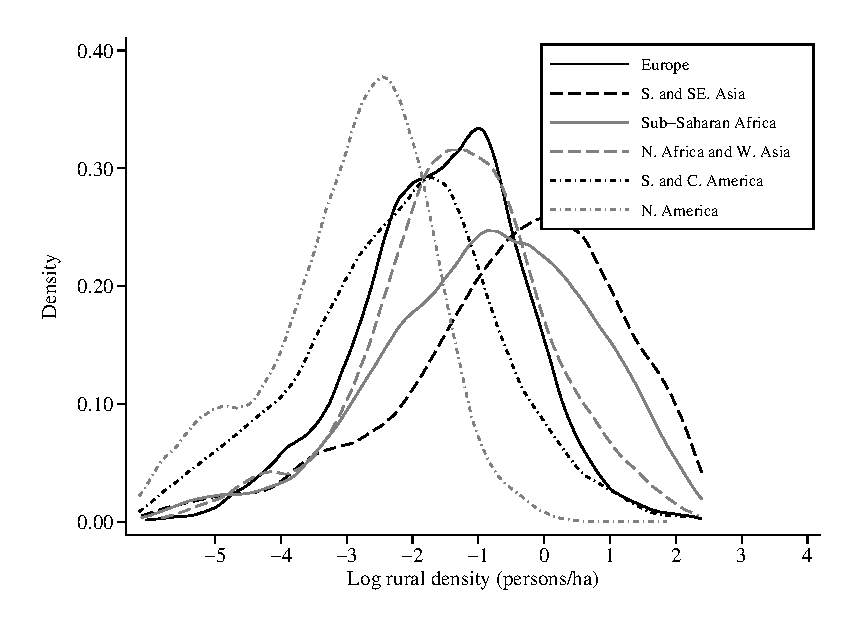
\includegraphics[width=1.0\textwidth]{fig_dens_rurd.eps}
\end{center}
\vspace{-.5cm}\singlespacing {\footnotesize \textbf{Notes}:Kernel density plot, Epanechnikov kernel, of the (log) rural density, $L_{Aisc}/X_{isc}$, at the district level, calculated by the authors using data from \citet{hyde31} for rural population. See text for details. See appendix for lists of exact countries included in each region.
}
\end{figure}

\clearpage

\begin{figure}[!htb]
\begin{center}
\caption{Density Plot of Caloric Yield ($A_{isc}$), by Region}
\label{FIG_dens_csi}
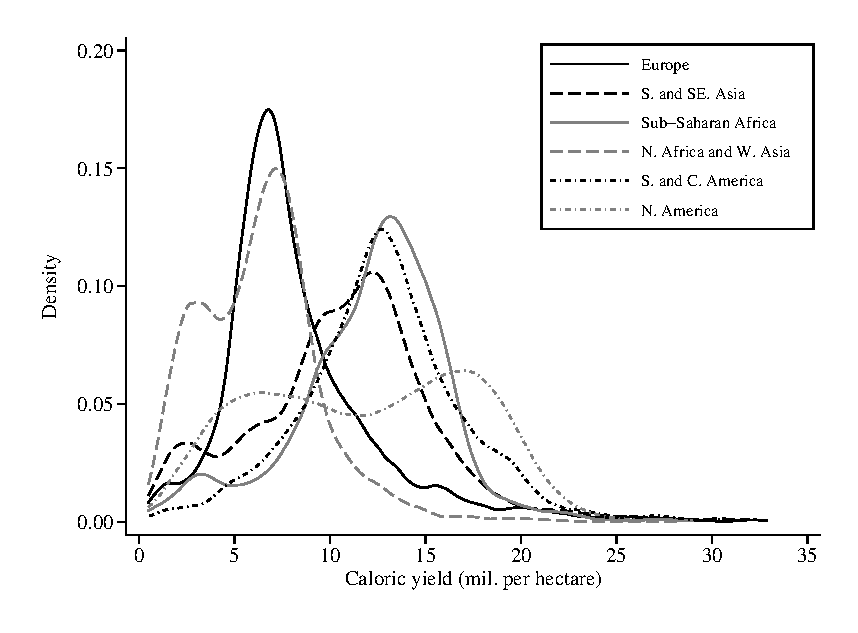
\includegraphics[width=1.0\textwidth]{fig_dens_csi.eps}
\end{center}
\vspace{-.5cm}\singlespacing {\footnotesize \textbf{Notes}: Kernel density plot, Epanechnikov kernel, of the caloric yield, $A_{isc}$, at the district level, calculated by the authors using data from \citet{galorozak2016}. See text for details. This measure sums the maximum calories available per grid cell within a district, then divides by total area of the district. See appendix for lists of exact countries included in each region.
}
\end{figure}


\clearpage


\begin{figure}[!htb]
\begin{center}
\caption{Caloric Yield and Rural Density, by Major Crop, 2000CE}
\label{FIG_beta_crop}
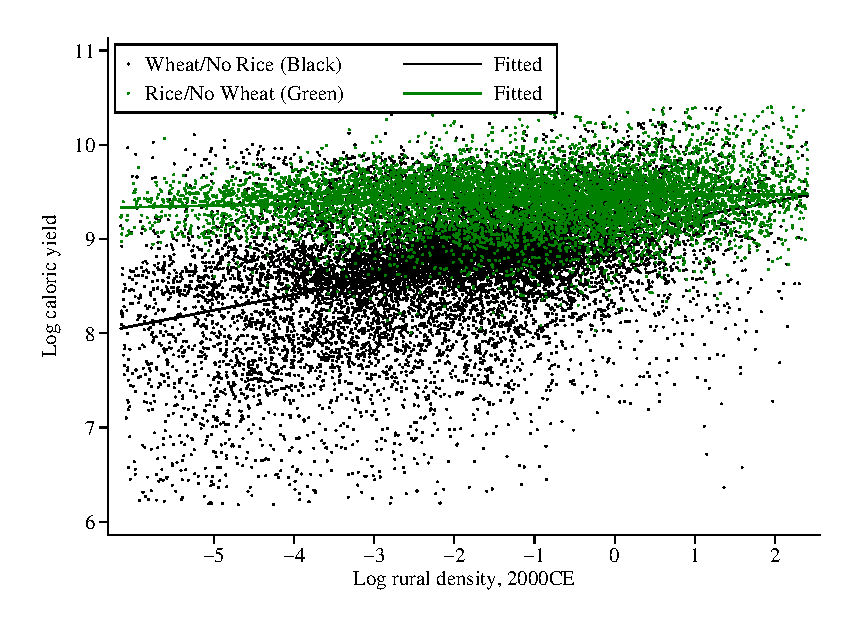
\includegraphics[width=1.0\textwidth]{fig_beta_crop.eps}
\end{center}
\vspace{-.5cm}\singlespacing {\footnotesize \textbf{Notes}: This figures shows the raw correlation of (log) caloric yield and (log) rural density for districts that are (a) suitable for wheat, but not for wet rice, and (b) suitable for wet rice but not for wheat. Rural population is from HYDE database \citep{hyde31}, and caloric yield is the author's calculations based on the data from \citet{galorozak2016}. The linear fits are from bivariate OLS regressions, without any fixed effects included. Based on equation (\ref{EQ_regress}), the slopes of these lines are estimates of $\beta$, the elasticity of agricultural output with respect to land.
}
\end{figure}

\clearpage

\begin{table}[!htb]
\begin{center}
\caption{Summary Statistics for District Level Data, 2000CE}
\label{TAB_summ}
{\small
\begin{tabularx}{\textwidth}{lXXXXXXX}
\midrule
 &      &            & \multicolumn{5}{c}{Percentiles:} \\ \cmidrule{4-8}
 & Mean & SD  & 10th    & 25th    & 50th & 75th & 90th \\
\midrule
Labor/land (persons/ha) &     0.73&     1.17&     0.04&     0.12&     0.32&     0.77&     1.86\\
Caloric yield (mil cals/ha) &    10.85&     4.89&     4.98&     7.17&    10.65&    13.86&    17.03\\
Log light density &    -2.82&     2.93&    -6.14&    -3.83&    -2.51&    -0.89&     0.35\\

\midrule
\end{tabularx}
}
\end{center}
\vspace{-.5cm}\singlespacing {\footnotesize \textbf{Notes}: A total of 32,862 observations for each variable (these come from 2,471 provinces in 154 countries). Caloric yield, $A_{isc}$ calculated by the authors using data from \citet{galorozak2016}. Rural density, $L_{Aisc}/X_{isc}$ calculated by the authors using data from \citet{hyde31} for rural population. Both caloric yield and rural density were trimmed at the 99th and 1st percentiles of their raw data prior to calculating the summary statistics in this table. Urbanization rate taken from \citet{hyde31}. Log mean light density derived from the Global Radiance Calibrated Nightime Lights data provided by NOAA/NGDC, as in \citet{hssw2016}. 
}
\end{table}

\clearpage

\begin{table}[!htb]
\begin{center}
\caption{Estimates of Malthusian Tightness, $\beta$, by Crop Suitability, 2000CE}
\label{TAB_beta_crops}
{\footnotesize
\begin{tabularx}{\textwidth}{lXXXXXX}
\midrule
\multicolumn{7}{l}{Dependent Variable in all panels: Log caloric yield ($A_{isc}$)} \\ \\
\multicolumn{7}{l}{Panel A: Samples defined by crop family (wheat vs. rice):} \\ \\
 & \multicolumn{2}{c}{By suitability:} & \multicolumn{2}{c}{By max calories:} & \multicolumn{2}{c}{By harvest area:}\\ \cmidrule(lr){2-3} \cmidrule(lr){4-5} \cmidrule(lr){6-7} 
 & Wheat & Rice & Wheat  & Rice  & Wheat  & Rice \\
 & Only & Only &  $>33\%$ & $>33\%$ & $>50\%$ & $>50\%$   \\
 & (1) & (2) & (3) & (4) & (5) & (6) \\
\midrule
Log labor/land ratio ($\beta_g$)&       0.239&       0.088&       0.218&       0.093&       0.220&       0.081\\
                    &     (0.045)&     (0.020)&     (0.039)&     (0.012)&     (0.049)&     (0.016)\\
\midrule
p-value $\beta_g=0$ &       0.000&       0.000&       0.000&       0.000&       0.000&       0.000\\
p-value $\beta_g=\beta_{Temp}$&            &       0.002&            &       0.002&            &       0.007\\
Countries           &          84&          76&          91&         101&          86&          78\\
Observations        &        9404&        7229&       15260&       14794&       10221&       10013\\
R-square (ex. FE)   &        0.24&        0.20&        0.21&        0.18&        0.23&        0.18\\

\midrule
\\
\multicolumn{7}{l}{Panel B: Samples with other restrictions (using suitability to distinguish crop families)} \\ \\
 & \multicolumn{2}{c}{Urban Pop. $<25K$:} & \multicolumn{2}{c}{Ex. Europe/N. Amer.:} & \multicolumn{2}{c}{Rural dens. $>$ 25th P'tile:}\\ \cmidrule(lr){2-3} \cmidrule(lr){4-5} \cmidrule(lr){6-7}
  & Wheat Only& Rice Only & Wheat Only& Rice Only& Wheat Only& Rice Only\\
 & (1) & (2) & (3) & (4) & (5) & (6) \\
\midrule
Residuals           &       0.257&       0.140&       0.223&       0.131&       0.215&       0.128\\
                    &     (0.022)&     (0.021)&     (0.032)&     (0.018)&     (0.021)&     (0.020)\\
\midrule
p-value $\beta=0$   &       0.000&       0.000&       0.000&       0.000&       0.000&       0.000\\
p-value $\beta=\beta_{Temp}$&            &       0.000&            &       0.009&            &       0.003\\
Countries           &          83&          75&          24&          70&          82&          66\\
Observations        &        7648&        6662&         824&        8826&        8084&        6611\\
Adjusted R-square   &        0.29&        0.24&        0.16&        0.14&        0.24&        0.20\\

\midrule
\end{tabularx}
}
\end{center}
\vspace{-.5cm}\singlespacing {\footnotesize \textbf{Notes}: Conley standard errors, adjusted for spatial auto-correlation with a cutoff distance of 500km, are shown in parentheses. All regressions include province fixed effects, a constant, and controls for the district urbanization rate and log density of district nighttime lights. The coefficient estimate on rural population density indicates the value of $\beta$, see equation (\ref{EQ_regress}). Rural population is from HYDE database \citep{hyde31}, and caloric yield is the author's calculations based on the data from \citet{galorozak2016}. Inclusion of districts in the regression is based on the listed criteria related to crop families. See text for all crops included in the wheat and rice families, and for details of the inclusion criteria.
}
\end{table}

\clearpage

\begin{table}[!htb]
\begin{center}
\caption{Estimates of Malthusian Tightness, $\beta$, by K{\"o}ppen-Geiger Zone, 2000CE}
\label{TAB_beta_kg}
{\footnotesize
\begin{tabularx}{\textwidth}{lXXXXXX}
\midrule
\multicolumn{7}{l}{Dependent Variable in all panels: Log caloric yield ($A_{isc}$)} \\ \\
\multicolumn{7}{l}{Panel A: Climate Zones} \\
 & Equatorial & Arid & Temperate & Snow  &     &   \\
 & (1) & (2) & (3) & (4) &  & \\
\midrule
Log rural density   &       0.111&       0.154&       0.169&       0.230\\
                    &     (0.015)&     (0.026)&     (0.017)&     (0.026)\\
\midrule
p-value $\beta=0$   &       0.000&       0.000&       0.000&       0.000\\
p-value $\beta=\beta^{Equa}$&            &       0.151&       0.007&       0.000\\
Countries           &          79&          56&          94&          40\\
Observations        &       11461&        2822&       13717&        6327\\
Adjusted R-square   &        0.11&        0.10&        0.15&        0.19\\

\midrule
\\
\multicolumn{7}{l}{Panel B: Precipitation Zones} \\
& Fully     & Dry         & Dry        &              &            & \\
& Humid & Summer & Winter & Monsoon & Desert & Steppe \\
 & (1) & (2) & (3) & (4) & (5) & (6) \\
\midrule
Log labor/land ratio ($\beta_g$)&       0.240&       0.215&       0.124&       0.125&       0.130&       0.147\\
                    &     (0.044)&     (0.063)&     (0.022)&     (0.039)&     (0.072)&     (0.029)\\
\midrule
p-value $\beta=0$   &       0.000&       0.001&       0.000&       0.001&       0.072&       0.000\\
p-value $\beta=\beta_{Humid}$&            &       0.739&       0.020&       0.043&       0.190&       0.072\\
Countries           &          78&          37&          67&          32&          20&          49\\
Observations        &       13545&        2373&        7695&        1267&         146&        1735\\
R-square (ex. FE)   &        0.17&        0.17&        0.15&        0.17&        0.17&        0.16\\

\midrule
\\
\multicolumn{7}{l}{Panel C: Temperature Zones} \\
    & Hot        & Warm        & Cool       & Hot      & Cold     &  \\
    & Summer & Summer & Summer & Arid & Arid &   \\
 & (1) & (2) & (3) & (4) & (5) &  \\    
\midrule
Log labor/land ratio ($\beta_g$)&       0.142&       0.226&       0.207&       0.140&       0.190\\
                    &     (0.021)&     (0.053)&     (0.076)&     (0.035)&     (0.046)\\
\midrule
p-value $\beta=0$   &       0.000&       0.000&       0.007&       0.000&       0.000\\
p-value $\beta=\beta_{Humid}$&            &       0.065&       0.405&       0.969&       0.254\\
Countries           &          57&          82&          18&          42&          25\\
Observations        &        8101&        9003&         340&        1230&         956\\
R-square (ex. FE)   &        0.20&        0.23&        0.20&        0.17&        0.21\\

\midrule
\end{tabularx}
}
\end{center}
\vspace{-.5cm}\singlespacing {\footnotesize \textbf{Notes}: Conley standard errors, adjusted for spatial auto-correlation with a cutoff distance of 500km, are shown in parentheses. All regressions include province fixed effects, a constant, and controls for the district urbanization rate and log density of district nighttime lights. The coefficient estimate on rural population density indicates the value of $\beta$, see equation (\ref{EQ_regress}). Rural population is from HYDE database \citep{hyde31}, and caloric yield is the author's calculations based on the data from \citet{galorozak2016}. Inclusion of districts is based on whether they have more than 50\% of their land area in the given K{\"o}ppen-Geiger zone. See text for details.
}
\end{table}

\clearpage
\begin{table}[!htb]
\begin{center}
\caption{Estimates of Malthusian Tightness, $\beta$, by Regions, 2000CE}
\label{TAB_beta_subregion}
{\footnotesize
\begin{tabularx}{\textwidth}{lXXXXX}
\midrule
\multicolumn{6}{l}{Dependent Variable in all panels: Log caloric yield ($A_{isc}$)} \\ \\
\multicolumn{6}{l}{Panel A} \\
 &          &         &             &  \multicolumn{2}{c}{Excl. China, Japan, Korea} \\ \cmidrule(lr){5-6}
 & North \& &         &              & South \&  & Central \&             \\
 & Western  & Eastern & Southern     & Southeast & West        \\
 & Europe   & Europe  & Europe       & Asia      & Asia      \\
 & (1) & (2) & (3) & (4) & (5) \\
\midrule
Log rural density ($\beta_g$)&       0.259&       0.287&       0.272&       0.152&       0.181\\
                    &     (0.036)&     (0.031)&     (0.041)&     (0.026)&     (0.024)\\
\midrule
p-value $\beta=0$   &       0.000&       0.000&       0.000&       0.000&       0.000\\
p-value $\beta=\beta_{NWEur}$&            &       0.539&       0.791&       0.017&       0.072\\
Countries           &          16&           9&           9&          13&          18\\
Observations        &        1684&        4821&        1137&        4312&        2878\\
R-square (ex. FE)   &        0.29&        0.34&        0.32&        0.21&        0.24\\

\midrule
\\
\multicolumn{6}{l}{Panel B} \\
 & Temperate & Tropical  & Tropical & South    & North    \\
 & Americas  & Americas  & Africa   & Africa   & Africa     \\
\midrule
Residuals           &       0.188&       0.113&       0.089&       0.134&       0.249\\
                    &     (0.030)&     (0.016)&     (0.014)&     (0.071)&     (0.014)\\
\midrule
p-value $\beta=0$   &       0.000&       0.000&       0.000&       0.059&       0.000\\
p-value $\beta=\beta_{NWEur}$&       0.133&       0.000&       0.000&       0.116&       0.827\\
Countries           &           5&          22&          39&           4&           5\\
Observations        &        3796&        9373&        3181&         198&        1220\\
R-square (ex. FE)   &        0.24&        0.12&        0.18&        0.27&        0.28\\

\midrule
\\
\multicolumn{6}{l}{Panel C} \\
 & All& Temperate & Sub-Tropical & & North \& \\
 & China & China  & China & Japan & South Korea  \\
 & (1) & (2) & (3) & (4) & (5) \\
\midrule
Log rural density   &       0.414&       0.518&       0.107&       0.155&       0.190\\
                    &     (0.083)&     (0.058)&     (0.026)&     (0.011)&     (0.061)\\
\midrule
p-value $\beta=0$   &       0.000&       0.000&       0.000&       0.000&       0.002\\
p-value $\beta=\beta^{NWEur}$&       0.102&       0.000&       0.001&       0.008&       0.309\\
Countries           &           1&           1&           1&           1&           2\\
Observations        &         266&         130&         136&        1039&         311\\
Adjusted R-square   &        0.25&        0.26&        0.21&        0.21&        0.21\\

\midrule

\end{tabularx}
}
\end{center}
\vspace{-.5cm}\singlespacing {\footnotesize \textbf{Notes}: Conley standard errors, adjusted for spatial auto-correlation with a cutoff distance of 500km, are shown in parentheses. All regressions include province fixed effects, a constant, and controls for the district urbanization rate and log density of district nighttime lights. See appendix for lists of exact countries included in each region. The coefficient estimate on rural population density indicates the value of $\beta$, see equation (\ref{EQ_regress}). Rural population is from HYDE database \citep{hyde31}, and caloric yield is the author's calculations based on the data from \citet{galorozak2016}. The countries included in each region can be found in the appendix.
}
\end{table}


\end{document}